
%%%%%%%%%%%%%%%%                                ~~~~~~~~~~~~~~~~~~~~~~~~~~~~~~~~~~~~~~~~~~~~~~~~~~
% CONDITIONALS %
%%%%%%%%%%%%%%%%                                ~~~~~~~~~~~~~~~~~~~~~~~~~~~~~~~~~~~~~~~~~~~~~~~~~~

\newif\ifPeerReview\PeerReviewfalse             % Whether to create the PeerReview version or
                                                % Journal version
\newif\ifFlatArchive\FlatArchivefalse           % Whether archive is flat (messy) or contain 
                                                % subfolders for graphics etc.
\newif\ifFloatAtEnd\FloatAtEndfalse             % Available in PeerReview mode:
                                                % Place floats at end of document?
\newif\ifTODO\TODOtrue                        % Use todo notes?

%%%%%%%%%%%%                                    ~~~~~~~~~~~~~~~~~~~~~~~~~~~~~~~~~~~~~~~~~~~~~~~~~~
% IEEEtran %
%%%%%%%%%%%%                                    ~~~~~~~~~~~~~~~~~~~~~~~~~~~~~~~~~~~~~~~~~~~~~~~~~~

\ifPeerReview
\documentclass[12pt,journal,draftclsnofoot,onecolumn]{IEEEtran}
% \newcommand\CLASSINPUTbaselinestretch{1.66}     % http://theoval.cmp.uea.ac.uk/~nlct/latex/thesis/node17.html
\else
\documentclass[journal]{IEEEtran}
\fi

% \RequirePackage[latin1]{inputenc}%              % Set input encoding (optionally latin1)
% \RequirePackage[T1]{fontenc}%                 % Set font encoding
% \usepackage[norsk]{babel}

% Single column review mode:
%\documentclass[12pt,journal,onecolumn]{IEEEtran}
%\newcommand\CLASSINPUTbaselinestretch{2}
%\RequirePackage{calc}
%\RequirePackage{fp} 
% Left margin = 1 inch + hoffset + oddsidemargin (or evensidemargin)
% Adding the 2cm gutter width to the odd/even side margins:
%\setlength\hoffset{0pt}
%\setlength\oddsidemargin{4cm}       % 4cm margins on the left side
%\addtolength\oddsidemargin{-1in}    % Subtract the initial 1 inch
%\setlength\textwidth{21cm-8cm}    % A4 width (21cm) minus margins on either side

%%%%%%%%%%%%%%%%%%%%%%%%%%%%%%                  ~~~~~~~~~~~~~~~~~~~~~~~~~~~~~~~~~~~~~~~~~~~~~~~~~~
% IEEE ''APPROVED'' PACKAGES %
%%%%%%%%%%%%%%%%%%%%%%%%%%%%%%                  ~~~~~~~~~~~~~~~~~~~~~~~~~~~~~~~~~~~~~~~~~~~~~~~~~~

\usepackage{cite}

\ifCLASSINFOpdf
   \usepackage[dvips]{graphicx}                 % Might not work. Use 'latex' instead of 
   \ifFlatArchive\else                          % 'pdflatex'
      \graphicspath{./gfx/}
   \fi
\else
   \usepackage[dvips]{graphicx}
   \ifFlatArchive\else
      \graphicspath{./gfx/}
   \fi
\fi

\RequirePackage[table,dvipsnames,svgnames]{xcolor}

\usepackage[cmex10]{amsmath}                    % cmex10 option to be IEEE explore compliant
\interdisplaylinepenalty=2500                   % Allows multiline equations to be broken

% \RequirePackage{amssymb}

\RequirePackage{array}

\ifCLASSOPTIONcompsoc
   \usepackage[caption=false,font=normalsize,labelfont=sf,textfont=sf]{subfig}
\else
   \usepackage[caption=false,font=footnotesize]{subfig}
\fi
\ifCLASSOPTIONcaptionsoff                       % IEEE promoted hack to turn off captions from the 
   \let\MYorigsubfloat\subfloat                 % subfloat package should the captionsoff option
   \renewcommand{\subfloat}[2][\relax]{\MYorigsubfloat[]{#2}} % be specified.
\fi

\ifFloatAtEnd
\ifCLASSOPTIONcaptionsoff                       % Places float at the end of the document when the
  \usepackage[nomarkers]{endfloat}              % captionsoff options is specified to IEEEtrans.cls
  \let\MYoriglatexcaption\caption               % (PeerReview mode)
  \renewcommand{\caption}[2][\relax]{\MYoriglatexcaption[#2]{#2}}
\fi
\fi

\usepackage{fixltx2e}                           % Fix some twocolumn float problems

%\usepackage{stfloats}                          % Allows: \begin{figure*}[!b]
                                                % (double column figures on top/bottom)

\usepackage{url}                                % Support for handling and breaking URLs

% NOTE: PDF hyperlink and bookmark features are not required in IEEE
%       papers and their use requires extra complexity and work.
\newcommand\MYhyperrefoptions{bookmarks=true,bookmarksnumbered=true,
pdfpagemode={UseOutlines},plainpages=false,pdfpagelabels=true,
colorlinks=true,linkcolor={black},citecolor={black},urlcolor={black},
pdftitle={An Optimized GPU Implementation of the MVDR Beamformer for Active Sonar Imaging},
pdfsubject={},
pdfauthor={Jo Inge Buskenes},
pdfkeywords={adaptive beamforming, beamforming, complexity, sonar, active}}%
\ifCLASSINFOpdf
   \usepackage[\MYhyperrefoptions,pdftex]{hyperref}
\else
   \usepackage[\MYhyperrefoptions,breaklinks=true,dvips]{hyperref}
   \usepackage{breakurl}                        % Allows 'dvips' driver to break links
\fi

%%%%%%%%%%%%%%%%%%%%%%%                         ~~~~~~~~~~~~~~~~~~~~~~~~~~~~~~~~~~~~~~~~~~~~~~~~~~
% ADDITIONAL PACKAGES %       
%%%%%%%%%%%%%%%%%%%%%%%                         ~~~~~~~~~~~~~~~~~~~~~~~~~~~~~~~~~~~~~~~~~~~~~~~~~~

% \ifPeerReview
% \let\OldIncludegraphics{\includegraphics}
% \usepackage{letltxmacro}
% \LetLtxMacro{\OldIncludegrsaphics}{\includegraphics}
% \renewcommand{\includegraphics}[2][]{\OldIncludegraphics[width=\linewidth, #1]{#2}}
% \fi

% % \makeatletter
% % \def\maxwidth{\ifdim\Gin@nat@width>\linewidth\linewidth
% % \else\Gin@nat@width\fi}
% % \makeatother
% % \let\Oldincludegraphics\includegraphics
% % \renewcommand{\includegraphics}[1]{\Oldincludegraphics[width=\maxwidth]{#1}}

\usepackage[maxfloats=40]{morefloats}
\newcounter{todoidx}
% \setcounter{todoidx}

\ifTODO
   \definecolor{todobackground}{rgb}{0.95,0.95,0.95}
   \setlength\marginparsep{1pt}
   \setlength\marginparwidth{35pt}
   \newlength\marginparwidthsmall
   \setlength\marginparwidthsmall{\marginparwidth}
   \addtolength\marginparwidthsmall{-7pt}
   \newcommand\todo[1]{%
      \addtocounter{todoidx}{1}%
      {\color{Red}\bf(\thetodoidx{})}%%\fbox{\bf\thetodoidx{}}}%
      \marginpar{%
         {\vspace*{-10pt}\color{Red}\fbox{\bf\thetodoidx{}}}\\%
         \fcolorbox{red}{todobackground}{\parbox{\marginparwidthsmall}{\scriptsize #1}}}}

   \newcommand\todopar[1]{\fcolorbox{red}{white}{\parbox{0.97\linewidth}{#1}}}
\else
%    \usepackage[disable]{./todonotes} 
   \newcommand\todo[1]{}
\fi

\newenvironment{narrow}[2]{%
\begin{list}{}{%
\setlength{\topsep}{0pt}%
\setlength{\leftmargin}{#1}%
\setlength{\rightmargin}{#2}%
\setlength{\listparindent}{\parindent}%
\setlength{\itemindent}{\parindent}%
\setlength{\parsep}{\parskip}}%
\item[]}{\end{list}}

\usepackage{float}

\definecolor{tabBlue}{HTML}{AACCFF}

%%%%%%%%%%                                      ~~~~~~~~~~~~~~~~~~~~~~~~~~~~~~~~~~~~~~~~~~~~~~~~~~
% MACROS %       
%%%%%%%%%%                                      ~~~~~~~~~~~~~~~~~~~~~~~~~~~~~~~~~~~~~~~~~~~~~~~~~~

% \DeclareMathOperator*{\argmin}{\text{arg}\;\text{min}}

\newcommand\Fig[1]{Fig.~\ref{#1}}

\newcommand\Grey[1]{{\color{Grey}#1}}
\newcommand\Red[1]{{\color{Red}#1}}
\newcommand\Blue[1]{{\color{Blue}#1}}
\newcommand\DarkBlue[1]{{\color{DarkBlue}#1}}
\newcommand\LightBlue[1]{{\color{LightBlue}#1}}
\newcommand\Brown[1]{{\color{Brown}#1}}
\newcommand\Green[1]{{\color{Green}#1}}
\newcommand\SeaGreen[1]{{\color{SeaGreen}#1}}
\newcommand\Yellow[1]{{\color{yellow}#1}}
\newcommand\Orange[1]{{\color{orange}#1}}

\newcommand\nn{\nonumber\\}

\newcommand\nmat[1]{\begin{matrix}#1\end{matrix}}
\newcommand\bmat[1]{\begin{bmatrix}#1\end{bmatrix}}
\newcommand\case[1]{\begin{cases}#1\end{cases}}
\newcommand\textbox[2]{\footnotesize\text{\parbox{#1}{\centering\emph{#2}}}}

\newcommand\rand{\text{rand}}
\newcommand\randn{\text{randn}}
\newcommand\rect{\text{rect}}
\newcommand\sinc{\text{sinc}}
\newcommand\tr{\text{tr}}
\newcommand\adj{\text{adj}}

% \newcommand\max{\text{max}}
\newcommand\argmin[1]{\text{arg}\;\underset{#1}{\text{min}}}

\newcommand\qqquad{\quad\qquad}
\newcommand\qqqquad{\qquad\qquad}

% \renewcommand\l[1]{\left#1}
% \renewcommand\r[1]{\right#1}

% {\text{\parbox{1.5cm}{\centering volume hyper- sphere}}}

%Keyword colouring:
\newcommand\kw[1]{#1}
\newcommand\parm[1]{#1}%\color{Black}#1\color{Black}}

\newcommand\of[1]{\scriptstyle(\parm{#1})\displaystyle}
\newcommand\df[1]{\scriptstyle[\parm{#1}]\displaystyle}
\newcommand\var[3]{#1_\text{#2}\of{#3}}

\newcommand\diag{\text{diag}}

% \raisebox{lift}[extend-above-baseline][extend-below-baseline]{text}
\newcommand\mt[1]{\text{\emph{#1}}} %mt = mathtext
\newcommand\mathnorm{\textstyle}
\newcommand\mathbig[1]{\displaystyle#1\mathnorm}
\newcommand\mathsmall[1]{\scriptstyle#1\mathnorm}
\newcommand\mathtiny[1]{\scriptscriptstyle#1\mathnorm}
\newcommand\sfrac[2]{\scriptstyle\raisebox{0.25pt}[0pt][0pt]{$\frac{#1}{#2}$}\mathnorm}
\newcommand\nfrac[2]{\textstyle\frac{#1}{#2}\displaystyle}

\newcommand\sumu[1]{\sum\limits^{#1}\;}
\newcommand\suml[1]{\sum\limits_{#1}\;}
\newcommand\sumb[2]{\sum\limits_{#1}^{#2}\;}

\newcommand\produ[1]{\prod\limits^{#1}\;}
\newcommand\prodl[1]{\prod\limits_{#1}\;}
\newcommand\prodb[2]{\prod\limits_{#1}^{#2}\;}

\newcommand\defeq{\overset{\underset{\mathrm{def}}{}}{=}}

%Math macros:
\newcommand\diff[2]{\frac{\kw{d}\;\textstyle #1\scriptstyle}{\kw{d\parm{#2}}}\displaystyle}
\newcommand\ddiff[2]{\frac{\kw{d^2}\;\displaystyle #1\scriptstyle}{\kw{d\parm{#2}}^2}\displaystyle}

\renewcommand\d[1]{\scriptstyle\kw{\;d\parm{#1}}\displaystyle}

% These commands are mutually exclusive. Remember to "renew" in v2.
\newcommand\intb[4]{\int\limits_{#3}^{#4} #1 \d{#2}} % \int{exp}{var}{from}{to}
\newcommand\intl[3]{\int\limits_{#3} #1 \d{#2}} % \int{exp}{var}{for all}
\newcommand\intu[2]{\int #1 \d{#2}} % \int{exp}{var}{for all}

\newcommand\T{^{\scriptscriptstyle T}}
\renewcommand\H{^{\scriptscriptstyle H}}

\renewcommand\vec[1]{\boldsymbol{#1}}
\newcommand\mat[1]{\boldsymbol{#1}}

\newcommand\Om{O_\text{m}}
\newcommand\Oa{O_\text{a}}
\newcommand\Nl{N_\text{l}}
\newcommand\Nk{N_\text{k}}
\newcommand\1{\vec 1}
\newcommand\I{\mat I}
\renewcommand*\a{\vec a}
\renewcommand*\i{\vec i}
\renewcommand*\k{\vec k}
\newcommand*\n{\vec n}
\newcommand*\p{\vec p}
\newcommand*\s{\vec s}
\newcommand*\w{\vec w}
\newcommand*\x{\vec x}
\newcommand*\y{\vec y}

\newcommand*\A{\mat A}
\newcommand*\B{\mat B}
\newcommand*\C{\mat C}
\newcommand*\E{\mat E}
% \renewcommand*\H{\mat H}
\renewcommand*\P{\mat P}
\newcommand*\eP{\mat{\hat P}}
\newcommand*\R{\mat R}
\newcommand*\Ri{\R^{-1}}
\newcommand*\eR{\mat{\hat R}}
\newcommand*\eRi{\hat{\mat R}\;\!^{-1}}
\newcommand*\Navg{N_\text{avg}}
\newcommand*\W{\mat W}
\newcommand*\X{\mat X}
\newcommand*\Xd{\X_{\!\Delta}}
\newcommand*\Y{\mat Y}

\renewcommand*\L{\mat \Lambda}
\newcommand*\U{\mat U}
% \renewcommand*\t{\mathtiny{^T}}
% \newcommand*\h{\mathtiny{^H}}
\renewcommand*\t{^T}
\newcommand*\h{^H}

\newcommand\D{\vec\nabla} %Del: Vector differential operator - nabla
\newcommand\Dx{\vec\nabla\times}
\newcommand\Dd{\vec\nabla\cdot}

\usepackage{tikz}
\usetikzlibrary{shapes,snakes}
\usepackage{amsmath,amssymb}
% \usepackage{datatool}
% \usepackage{glossaries}

\newenvironment{outline}
{\begin{itemize}}
{\end{itemize}}

%    \definecolor{todobackground}{rgb}{0.95,0.95,0.95}
%    \setlength\marginparsep{3pt}
%    \setlength\marginparwidth{42pt}
%    \newlength\marginparwidthsmall
%    \setlength\marginparwidthsmall{\marginparwidth}
%    \addtolength\marginparwidthsmall{-7pt}
%    \newcommand\todo[1]{%
%       \addtocounter{todoidx}{1}%
%       {\color{Red}\fbox{\bf\thetodoidx{}}}%
%       \marginpar{%
%          {\vspace*{-10pt}\color{Red}\fbox{\bf\thetodoidx{}}}\\%
%          \fcolorbox{red}{todobackground}{\parbox{\marginparwidthsmall}{#1}}}}
% 

% correct bad hyphenation here
% \hyphenation{op-tical net-works semi-conduc-tor}

%%%%%%%%%%%%                                    ~~~~~~~~~~~~~~~~~~~~~~~~~~~~~~~~~~~~~~~~~~~~~~~~~~
% GLOSSARY %
%%%%%%%%%%%%                                    ~~~~~~~~~~~~~~~~~~~~~~~~~~~~~~~~~~~~~~~~~~~~~~~~~~

% \makeglossaries
% \newglossaryentry{ASIC}{name={ASIC},
                  description={Application Specific Integrated Circuit} } 
                  
\newglossaryentry{ATR}{name={ATR},
                  description={Automatic Target Recognition} } 

\newglossaryentry{CPU}{name={CPU},
						description={Central Processing Unit} } 

\newglossaryentry{GPGPU}{name={GPGPU},
						description={General Purpose Graphics Processing Unit} } 

\newglossaryentry{GPU}{name={GPU},
						description={Graphics Processing Unit} } 
					
\newglossaryentry{MVDR}{name={MVDR},
						description={Minimum Variance Distortionless Response} } 

%%%%%%%%%%%%%%%%%%                              ~~~~~~~~~~~~~~~~~~~~~~~~~~~~~~~~~~~~~~~~~~~~~~~~~~
% DOCUMENT START %
%%%%%%%%%%%%%%%%%%                              ~~~~~~~~~~~~~~~~~~~~~~~~~~~~~~~~~~~~~~~~~~~~~~~~~~

% \usepackage{yfonts}


\begin{document}


\title{An Optimized GPU Implementation of the MVDR Beamformer for Active Sonar Imaging}

\author{Jo~Inge~Buskenes, %
        Jon~Petter~\AA{}sen, %
        Carl-Inge~Colombo~Nilsen, %
        Andreas~Austeng%
\thanks{J. I. Buskenes, C.-I. C. Nilsen and A. Austeng are with the Department of Informatics, University of Oslo, Norway.}%
\thanks{J. P. \AA{}sen is with MI-Lab, Norwegian University of Science and Technology, Trondheim, Norway.}% <-this % stops a space
% \thanks{Manuscript received April 19, 2005; revised January 11, 2007.}
}

% The paper headers
\markboth{IEEE Journal of Oceanic Engineering}%
{A Robust and Optimized GPU Implementation of the MVDR beamformer}

% Publishers ID mark:
%\IEEEpubid{0000--0000/00\$00.00~\copyright~2007 IEEE}

% use for special paper notices
%\IEEEspecialpapernotice{(Invited Paper)}

% for Computer Society papers, we must declare the abstract and index terms
% PRIOR to the title within the \IEEEcompsoctitleabstractindextext IEEEtran
% command as these need to go into the title area created by \maketitle.
\IEEEcompsoctitleabstractindextext{%
\begin{abstract}
% Two limiting factors of modern phased array sonar imaging systems are the angular resolution and contrast. Adaptive beamformers target these limitatitons by weighting sensors dynamically to fit the impinging wavefield.

The Minimum Variance Distortionless Response (MVDR) beamformer has recently been proposed as an attractive alternative to conventional beamformers in active sonar imaging. Unfortunately, it is very computationally complex because a spatial covariance matrix must be estimated and inverted for each image pixel. This may discourage its use unnecessarily in sonar systems which are continuously being pushed to ever higher imaging ranges and resolutions.

In this study we show that for active sonar systems up to 32 channels, the computation time can be significantly reduced by performing arithmetic optimizations, and by implementing the MVDR on a Graphics Processing Unit (GPU). We point out important hardware limitations for these devices, and assess the design in terms of how efficiently it is able to use the GPU's resources. On a quad-core Intel Xeon system with a high-end Nvidia GPU, our GPU implementation renders more than 1\;Mpx/s. This represents a speedup of more than two orders of magnitude over our initial single threaded implementation in C. This enables real-time processing of sonar data, and makes the MVDR a viable alternative to conventional methods in practical systems.
% If the HISAS1030 was attached to a platform traveling at 1.8m/s, creating full-coverage sectorscan images in real-time would be possible with this performance.

% We benchmarked optimized implementations of the MV beamformer in Matlab and C, running on a quad-core Intel Xeon E5620, and in CUDA running on a high-end nVidia card. The beamformers operated on data from the 32x4 element Kongsberg Martime HISAS1030 sonar, using a conservative set of robustification parameters. 
%The CPU would then be free to take on the rest of the beamforming as well.
\end{abstract}

% Keywords (normally not used for peer reviews)
\ifPeerReview\else
\begin{IEEEkeywords}
Adaptive beamforming, MVDR, Capon, sonar, active sonar, GPU, graphics processing unit, complexity.
\end{IEEEkeywords}
\fi}
% \fi

% make the title area
\maketitle

% This command fixes abstract positioning for compsoc articles:
\IEEEdisplaynotcompsoctitleabstractindextext

% (Optional) Add some extra info on cover page of peer review papers:
% \ifCLASSOPTIONpeerreview
% \begin{center} \bfseries EDICS Category: 3-BBND \end{center}
% \fi

% Insert page break and insert second title (peer review mode)
\IEEEpeerreviewmaketitle

\maketitle

\section{Introduction}

% Images from a phased array active sonar system are formed in the post-processing by focusing on one pixel at a time. This is achieved by delaying and weighting each of the array's channels, providing coarse and fine adjustments to the region of focus, respectively. This is commonly referred to as beamforming. Assuming far-field conditions, the delays are usually chosen to steer the pixel of interest to broadside, and the weights chosen to reject the noise impinging on the array from non-broadside directions.
% 
% The algorithm responsible for carrying out this task is referred to as a beamformer. Depending on whether data is evaluated when choosing a suitable set of delays and weights, beamformers can be branded either conventional or adaptive. A good example of the former is the The Delay-and-Sum (DAS) beamformer, which - as the name implies - simply delay the sensor channels appropriately prior to summing them up. Applying various weight sets, or windows, to the data prior to summation allows the lateral \gls{SNR} to be improved, but at the inevitable expense of a deteriorated lateral resolution. \todo{aka. the curse of physics.}
% 
% The Minimum Variance Distortionless Response (MVDR) (or \gls{MVDR}) beamformer, have the potential to overcome this limitation. While ensuring unit gain in the look direction, it computes the set of weights that minimizes the energy accumulated by the array from other directions. In other words, whenever the distribution of noise and interference is primarily focused around specific angles, an array response with a high degree of suppression at these angles are chosen, resulting in an image with a lateral \gls{SNR} and resolution superior to anything the \gls{DAS} can come up with.


% 
% In active sonar imaging the constrast and resolution can be improved by the use of adaptive beamforming. 
% 
% Adaptive beamforming 
% A critical part in the sonar image formation is the 
% The image quality is mainly limited by beampattern of the imaging arrays.  resolution and noise suppression
% 
% The quality of sonar images 
% 
% An essential part of a sonar imaging system is the beamformer. 
% 
% 
% A sonar image is typically formed by using receive beamforming to focus on one pixel at a time. The beamformer's ability to suppress interference   to focus on one pixel at the time. How well a pixel value is estimated, and thus how 
% 
% A sonar image is built one pixel at the time the 
% 
% The image quality of a sonar system will depend on the imaging arrays ability to focus in 
% 
% 
% 
% Forming images done by combining data from multiple receivers in a way that to obtain focus on one pixel at the time, and assigning the output value to the intensity of that pixel. The 
% 
% Most modern active sonar systems employ phased arrays to 
% The basic way of a sonar image was formed 
% 
% A sonar system's ability to 
% 
% Adaptive beamforming has 
% 
% The image quality 
% 
% To improve the image quality of 
% 
% In high resolution sonar imaging the 
% 
% The image 
% 
% 
% In a typical sonar imaging scenario an encoded signal is transmitted to highlight a surface of interest, and the reflected wavefield sampled using a receiver array. A image is then formed in the post-processing by coherently combining the receiver outputs to focus at one pixel at the time. The principle of adjusting the arrays focus is commonly referred to as beamforming, and involves assigning suitable delays and weights to the array's channels.
% 

% A sonar image is typically formed by using receive beamforming to focus on one pixel at a time.   The image resolution and contrast The image quality The quality of active sonar images depend - amoung other things - on the beamformer's ability to suppress interference  resolution and constrast
% 
% A sonar image is typically formed by using receive beamforming to focus on one pixel at a time. The quality of the final image will depend on the beamformer's ability to suppress interference and noise from off-pixel.    to focus on one pixel at the time. How well a pixel value is estimated, and thus how
% 
% 
% In conventional active sonar imaging systems 
% 
% Various methods have been applied to active sonar imaging. One of these methods, 
% 
%  eamforming techniques have been applied in several fields to improve image. methods can be applied to 
% 
% Most active sonar imaging systems are based on conventional beamforming methods. These are robust and simple, but does not take the incoming wavefield into account. offer  in the image formation process. While being inherently robust, these methods 
% 
% 
% With the ever increasing processing power found in modern computers 
% 
% As the processing power of todays modern computer systems keeps improving the feasibility of 
% 
% As the processing power of modern computer systems keep improving, the use of data adaptive methods in various imaging fields. 

\IEEEPARstart{D}{ata} driven methods have been introduced in various imaging fields over the years in attempts to improve image quality. One such method is the Minimum Variance Distortionless Response (MVDR) beamformer. When compared to conventional methods, MVDR is often able to improve image contrast and resolution, as shown in e.g. radar~\cite{Benitz1997}, ultrasound~\cite{Synnevag2007}, and active sonar~\cite{Blomberg2012a,Blomberg2011,Dursun2009,Lo2004}.

Despite its inherent potential, the MVDR beamformer has yet to see widespread adoption in the active sonar field. There may be several reasons for this. For one, the method is not inherently robust, and may suffer from a phenomenon called signal cancellation in active systems~\cite{Widrow1982}. Another reason is that in its original form, the computational complexity is cubic with the number of channels, O($M^3$), while conventional beamformers are at O($M$). This is because a spatial covariance matrix is estimated and inverted for each image pixel.

% Robustification:
% R estimate accuracy vs. dynamic trackability: (1) Trade observation time for bandwidth (2) Partial adaptiveness (less degrees of freedom than channels) (3) Quadratic constraint on sensor weights to limit the norm to some preset value.
% -  
To ensure MVDR robustness, the litterature suggests combining means such as temporal and spatial averaging, and regularization~\cite{VanTrees2002,Kailath1985}. The complexity issue, on the other hand, can be handled by introducing well-founded approximations. For instance, some studies assume data stationarity which allows the formation of a Toeplitz-structured covariance matrix that is simpler to invert~\cite{Asl2012a,Jakobsson2000}. Other studies perform MVDR beamforming in beamspace (the spatial frequency domain), which can be considered sparse due to the limited angular extent of the received beam~\cite{VanTrees2002,Nilsen2009}. Exploiting this can lead to considerable performance improvements, especially in high channel count systems.

% Some low complexity approximations to the MVDR beamformer is also available, such as the Low Complexity Adaptive (LCA) beamformer, 

% Such devices can often this by combining up to thousands of computing cores that each performs modestly, but combined performs impressively. 

% We will show that by exploiting symmetry and avoiding unnecessary computations, the spatial averaging will also aid in reducing the overall arithmetic complexity\todo{make sure this is shown clearly somewhere}. for Unlike other work, which focus modifying or transforming\todo{get low channel count in, as it makes a case against the other solutions.} We make no approximations, but rather stay with a textbook example of the method that handle complex basebanded data\todo{misplaced?}.

% Other work (keywords: mvdr, capon, computation, efficient, complexity):
% - Partially adaptive beamforming. DAS on non-overlapping subarrays, then MVDR \cite{Swingler1999a}.
% - Beamspace / frequency based methods.
% - Low complexity. PCA + LC. 
% - Systolic arrays. Radar \cite{Ward1984} 
% - Toeplitz. \cite{Yapanel} Spectrum estimation - speech recognition. 
% 
% Us:
% - Aim for the GPU. Simple is often better.
% - Therefore: Optimize the standard MVDR chain.
% 1. Reduce arithmetic instructions
% 2. Implement for full utilisation of the arithmetic throughput on the GPU.
% 
% (Made partially adaptive by employing subarray averaging to reduce degrees of freedom to L.)


In this work, we show that such approximations may not be necessary for sonar systems up to 32 channels, since here the computation time can be reduced by 1-2 orders of magnitude by implementing MVDR on a Graphics Processing Unit (GPU). Similar work may be found in e.g. medical ultrasound imaging, where Chen \emph{et al.} have demonstrated a GPU implementation of the MVDR that operates on real valued data~\cite{Chen2011,Chen2011a}. While this implementation is fast, the real valued data constraint does not allow the creation of asymmetric and shifted responses, and hence prevents the MVDR's potential to be fully reached. Our implementation is not restricted in this manner. In related work, we investigated using the same MVDR GPU implementation in cardiac ultrasound imaging~\cite{Asen2012,Asen2013}, and in active sonar imaging we have compared the performance of this implementation to comparable adaptive methods~\cite{Buskenes2013a}.

This article is outlined as follows: In section \ref{methods} we introduce the concept of adaptive beamforming and provide details on the MVDR method. Then in \ref{maptogpu} we investigate the complexity issue, discuss means for reducing arithmetic complexity, and detail an implementation that makes efficient use of the GPU's parallel resources. The final design is assessed in \ref{images_and_benchmarks}-\ref{discussion}, where we provide benchmarks, comparisons with similar CPU implementations, and measures of how efficiently our implementation makes use of the GPU's resources.

%  Furthermore, by implementing it on a modern \gls{GPU} we have gained a speedup of around 2 orders of magnitude compared to an optimized single-thread implementation in C.

% These devices have in recent years emerged as a flexible and highly potent parallel technology well suited for many DSP tasks, and are available off-the-shelf at reasonable prices\todo{skip this?}.


% These devices have in recent years emerged as a flexible and highly potent parallel technology well suited for many DSP tasks, and are available off-the-shelf at reasonable prices.

% Yay or nay? $\Rightarrow$ GPU ultrasound (\cite{So2011,Chen2011}). Complex data, all robustification techniques.


% - Adaptive beamformers offers image quality edge, but are usually computationally complex.
% - Who's tried before?
% - We: Active sonar MVDR, GPU, high performance.


\section{Methods}\label{methods}

Consider a sonar imaging scenario where an encoded signal is transmitted to highlight a surface of interest, and assume that the backscattered wavefield is properly sampled using a uniform linear array of receivers. An image can then be formed by coherently combining the receiver outputs to focus at one angle at the time. The principle of adjusting the array's focus in range and direction is commonly referred to as beamforming, and involves assigning suitable delays and weights to the array's channels.


\subsection{Beamforming}

\ifPeerReview
\begin{figure}[H]\centering
\includegraphics[width=0.8\linewidth]{gfx/buske1.eps}
\else
\begin{figure}[!t]\centering
\includegraphics[width=\linewidth]{gfx/beamforming.eps}
\fi%
\caption{Beamforming principle. Signal signature is first removed by matched filtering. Then - prior to summation - a suitable set of delays, $\Delta$, and weights, $w$, are applied to focus on a pixel of interest at angle and range ($\theta,n$).}\label{beamforming}
\end{figure}
Let the receiver be an $M$ element uniform linear array, and assume that the signature of the transmitted signal has been removed by a matched filter (Fig. \ref{beamforming}). Further assume that the array channels are digitally delayed to focus at a pixel with azimuth angle $\theta$ and range sample $n$, such that the delayed data from the $m$th channel can be expressed as $x_m[\theta,n]$. To simplify notation, we make the dependence on $\theta$ implicit from now on. 

By definition the beamformer output $z[n]$ can now be expressed as the weighted sum of all the delayed data samples:
\begin{align}
z[n] = \w\H[n]\x[n] = \bmat{w_0[n]\\w_1[n]\\\vdots\\w_{M-1}[n]}^H \bmat{x_0[n]\\x_1[n]\\\vdots\\x_{M-1}[n]},\label{z}
\end{align}
where $w_m$ is the weight factor assigned to channel $m$. With static weights this would be referred to as the conventional delay-and-sum (DAS) beamformer. A large variety of weighting functions exists here for trading lateral resolution for improved noise suppression (contrast), but one always ends up with a compromise between the two~\cite{Harris1978}.

Various adaptive beamformers target this limitation by allowing the weights to change for each pixel to better fit the dynamic nature of the incoming wavefield. In other words, they attempt to use the \emph{a priori} information present in the data to improve image quality. The MVDR beamformer is one such method. It finds the set of complex weights that minimizes the beamformer's expected output power, while ensuring unity gain in the look direction~\cite{Capon1969}. This is a convex optimization problem that can be solved using Lagrange multipliers to yield the solution:
\begin{gather}
\vec w[n] = \frac{\Ri[n]\1}{\1\T\Ri[n]\1},\label{weights}
\end{gather}
where $\1$ is a row vector of ones that represents broadside steering, and $\R=E\{\x[n]\x\H[n]\} \in\mathbb{C}^{M,M}$ is the spatial covariance matrix for the full array. Since $\R$ is unknown, we estimate it by computing a sample covariance matrix $\eR$. In this computation we will perform some degree of \emph{spatial averaging} to avoid signal cancellation, \emph{temporal averaging} to maintain true speckle statistics~\cite{Synnevag2009a}, and \emph{diagonal loading} to improve robustness to parameter errors ~\cite{Cox1987,Maksym1979}. Combined, these steps will also ensure a numerically well conditioned $\eR$.

To form $\eR$ we will first compute an intermediate sample covariance matrix $\breve{\R}$, which we form using temporal and spatial averaging. To do this we need to segment our array into subarrays. If we let $x_l[n]$ represent the data vector from subarray $l$,
\begin{gather}
\x_l[n] = \bmat{x_l[n] & x_{l+1}[n] & \dots & x_{l+L-1}[n]}\T,
\end{gather}
then $\breve{\R}$ can be calculated as:
\begin{gather}
\breve{\R}[n] =  \frac{1}{N_K N_L} \sumb{l=0}{M-L}\sumb{n'=n-K}{n+K} \x_l[n]\x_l\H[n] \in\mathbb{C}^{L,L},\label{spatialR}
\end{gather}
where $N_K = 2K+1$ is the number of temporal samples to perform averaging over, and $N_L = M-L+1$ is the number of subarrays.

The final estimate $\eR$ is found by adding a fraction $d$ of the total power of $\breve{\R}[n]$ to its diagonal~\cite{Synnevag2007}:
\begin{align}
\eR[n] = \breve{\R}[n] + \I \frac{d}{L} \tr\{\breve{\R}[n]\},\label{finalR}
\end{align}
where $\I$ is an identity matrix, $\tr\{\cdot\}$ represents the matrix trace operation, and $\tr\{\breve{\R}[n]\}$ is an estimate of the energy received from this pixel.

Note how subarray averaging led to a size reduction of $\eR$ from $\mathbb{C}^{M,M}$ to $\mathbb{C}^{L,L}$, and hence will produce an $L$-element weight set when substituted into (\ref{z}). This weight set is applied to all the subarrays, prior to computing the beamformer output as in (\ref{z}). Or, equivalently, we may apply the weight set to the sum of all the subarrays:
\begin{align}
z[n] = \w\H[n] \sumb{l=0}{M-L} \x_l[n].\label{finalZ}
\end{align}
\ifPeerReview
\begin{figure}[!t]\centering
\includegraphics[width=.8\linewidth]{gfx/buske2.eps}
\else
\begin{figure}[!t]\centering
\includegraphics[width=\linewidth]{gfx/implementation.eps}
\fi%
\caption{MVDR beamforming. For each pixel in range and azimuth,\newline
1. an $L\times{}L$ sample covariance matrix $\eR$ is computed, \newline
2. the term $\eR^{-1}\1$ is found using a linear equation solver,\newline
3. and the beamformer output $z$ is computed from (\ref{finalZ}), where $\w$ is found by substituting $\eR^{-1}\1$ into (\ref{weights}). } \label{mvdr_beamforming}
\end{figure}
% \begin{figure}[!t]\centering
% \includegraphics[width=\linewidth]{gfx/algorithm_structure.eps}
% \caption{MVDR beamforming. First a spatial covariance matrix is estimated from the delayed data (\ref{spatialR}-\ref{finalR}), then the weights are computed (\ref{weights}) and finally applied to the delayed channel data (\ref{z}).}
% \label{implementation}
% \end{figure}
As summarized in Fig. \ref{mvdr_beamforming}, the MVDR method is applied to each pixel independently, by:
\begin{enumerate}
\item computing the sample covariance matrix $\eR$ in (\ref{finalR}),
\item computing $\eRi\1$ in (\ref{weights}), and
\item computing the beamformer output $z$ in (\ref{finalZ}).
\end{enumerate}
% This is illustrated in .
% \begin{figure}[!t]\centering
% \includegraphics[width=\linewidth]{gfx/buildR-complex_data-average.eps}
% \caption{.}\label{complexity}
% \end{figure}
Next we will evaluate these steps in terms of arithmetic complexity, and then discuss their mappability to parallel hardware.

\subsection{Computational Complexity}

 
% Computing and inverting $\eR$ is by far the most computationally intensive tasks in MVDR beamforming. This 

If we neglect spatial and temporal averaging, then the computation of $\eR$ is reduced to a single outer product with complexity of O($M^2$), and the inversion is then of O($M^3$). This might lead us to believe that the inversion step is by far the most complex. But if we implement spatial and temporal averaging as in (\ref{spatialR}), then computing $\eR$ is of O($N_K N_L L^2$) and the inversion of O($L^3$). Computing $\eR$ is now the most complex operation whenever $N_LN_K>L$.
\ifPeerReview
\begin{figure}[!t]\centering
\includegraphics[width=.8\linewidth]{gfx/buske3.eps}
\else
\begin{figure}[!t]\centering
\includegraphics[width=\linewidth]{gfx/mvdr_complexity.eps}
\fi%
\caption{Per-pixel computational complexity of the steps in MVDR beamforming (prior to any optimizations). To avoid signal cancellation in an active sonar system we usually set $L<\frac{M}{2}$, in which region the computation of $\eR$ dominates in terms of arithmetic complexity, especially when performing temporal averaging.}\label{mvdr_complexity}
\end{figure}
To visualize these relations, and include the effects of using complex numbers, we set up complexity formulas that account for the total number of arithmetic operations for each step in the MVDR process (see appendix \ref{mvdr_formulas}). We only excluded diagonal loading performed in the computation of $\eR$, and partial pivoting used in the inversion step, since these operations contribute marginally to the end result. The entire range of possible subarray sizes from $L\in[1,M]$ was finally evaluated, with temporal averaging set to $K\in\{0,1,2\}$, and the number of channels set to $M\in\{8,16,32\}$. The results are shown in \Fig{mvdr_complexity}.

We note how the computation of $\eR$ completely dominates at smaller subarray sizes, that solving $\eRi\1$ only plays a notable role for larger array and subarray sizes, and that the computation of $z$ has a negligible impact on computation time. Also notice how temporal averaging comes with a high computational penalty. This is because building $\eR$ is heavy on complex multiplications, which require 3 times as many arithmetic instructions as a complex addition, and a lot of these are repeated unnecessarily.



% Not corrected for fused multiply accumulate

% Also, the need for partial pivoting has been ignored, as we ensure a numerically well conditioned $\eR$ by applying diagonal loading. Since this is the most common scenario, we will have a thorough look at how it can be optimized.

% and does not take into that does not  feasibility parallel decomposition  memory consumption.



\section{Mapping the MVDR to a GPU}\label{maptogpu}

% \begin{itemize}
% \item Keep delay step on CPU, as this is a common step in all beamforming
% \item Increasing matrix size reduces the number of threads per block, since the entire matrix must be in shared memory. 1 matrix 72x72 complex (8 bytes) max per block - 72 threads. same as 207 5x5 matrixes, 5*207=1036 threads. max threads in block 512.
% \end{itemize}

% An important feature of MVDR beamforming, and with beamforming in general, is that each pixel can be computed independently and in an identical fashion. Considering that sonar images often end up having millions of pixels, this makes a compelling case for investigating technologies that support massive data level parallelism. The technology that does this best is perhaps Graphics Processing Units (GPUs). These chips contain up to thousands of small computation cores, which combined deliver superior peak floating point performance compared multi-core systems such as CPUs.

An important feature of MVDR beamforming, as with beamforming in general, is that each pixel can be computed independently and in an identical fashion. Furthermore, a typical sonar image may contain millions of pixels. This represents a level of data parallelism that appears very well suited for a massively parallel architecture such as the GPU.

We decided to investigate the feasibility of running MVDR on a GPU by mapping it to a Nvidia GeForce Quadro 6000. This is a high-end Compute Unified Device Architecture (CUDA) enabled GPU based on Nvidia's Fermi architecture. The code was written in Nvidia's ``C for CUDA'' framework. We believe that GPUs from AMD, or the cross-platform OpenCL framework from the Khronos group, are equally attractive alternatives, but comparing them is beyond the scope of this study.

To use Nvidia's own terminology, the Quadro 6000 is comprised of 14 streaming multiprocessors (SMs), each having 32 CUDA cores that execute a common program called a kernel. Combined these cores deliver a peak performance of more than 1\;Tflop/s (appendix \ref{throughput}). In practice this performance is hard to obtain, but one can get fairly close by balancing the load evenly on all cores, and by trying to avoid that some cores are forced to idle due to a pending data transfer or thread synchronization. As the steps in the MVDR method require different strategies for achieving this, we have designed a different kernel and configuration for each of them. We will pay particular attention to building $\eR$, since the potential for gaining overall speedups are greatest here.

%  this assumes that the implementation is solely bound by arithmetic throughput.  r bound by memory bandwidth, arithmetic latency or arithmetic bandwidth.  or  is solely bound by processing power.   These cores need to be kept busy if we are to That make for a total of 448 CUDA cores which we need to keep busy if we want to tap the full potential. 

\ifPeerReview
\begin{figure}[t]\centering
\includegraphics[width=.8\linewidth]{gfx/buske4.eps}
\else
\begin{figure}[t]\centering
\includegraphics[width=\linewidth]{gfx/mvdr_build_R.eps}
\fi%
\caption{Step 1: Building $\eR$. This is a visualization of how $\eR$ could be built in a case with $M=5$ sensors, with subarray size $L=3$ and temporal averaging set to $K=1$. Here $\R'_{l}$ is the sample covariance matrix for the $l$th subarray, and $\breve{\R}$ is the average of $N_K$ of these. Note that instead of performing the temporal sum last as here, one could take more temporal samples into consideration in the computation of each $r_{ij}$.}\label{mvdr_build_R}
\end{figure}


% \todo{Another shitty GPU transition}
% Before proceeding we should make a quick note on the GPU memory. Note that to obtain the best possible performance, we need to make sure that CUDA threads find the data they need in cache or registers most of the time. Only these two memory types have a high enough bandwidth to promote sustained maximum utilisation of all CUDA cores. Unfortunately, they are a sparse resource. 

% This makes it apparent that computing one pixel per thread is not a feasible solution. \todo{...}

% When optimizing an algorithm for speed, it is if of importance to know whether an algorithm is bound by computations or memory. One way to get an approximate idea of this is to compute the ratio of peak arithmetic throughput to peak memory throughput of the in the target platform, and compare this ratio to the ratio of arithmetical operations to memory operations in the algorithm. 

% follow collective access patterns to memory.

% At first glance, it might seem like a good idea to compute one pixel per CUDA core. Each pixel is computed using the same instructions, and without any exchange of data. However, this approach is unfeasible due to the limited cache and register memory available to each thread. One could resolve to using the slower GDDR5 memory, but this would largely mitigate the performance gain and defeat the purpose of using a GPU in the first place.

%Bandwidth becomes crucial, as getting data in to the cores and out again must happen i a frantic pace. %the feeding all these cores with data and harvesting the result

% To effectively harness the computing potential of a GPU we need to make sure all computing cores stays busy most of the time. 

% Memory latency can be hidden in two ways. One is to keep a lot of threads queued up on each SM at all times, such that when some threads perform memory operations other threads can be scheduled to run instead. This is referred to as data level parallelism (DLP). Alternatively, or preferrably in addition, the designer may promote instruction level parallelism (ILP) by letting subsequent instructions in a thread be independent. While ILP can be very effective when done correctly, DLP is generally simpler to design for.
% 
% In the CUDA framework, the threads on an SM is managed through a software abstraction call a compute block. The block is a 3 dimensional grid where each element correspond to a thread that is scheduled to be executed on the SM at some point.

% load balancing
% - distribute load - optimize symmetry
% - avoid branching
% 
% memory latency hiding
% - make threads use high bandwidth memory
% - hide latency with dlp, ilp, or both
% 
% thread sync hiding
% - queue blocks up on an sm

%This is referred to as a single-program, multiple-data (SPMD) architecture\todo{malplaced}.

 %An SM is a single-program multiple-data (SPMD) processor, meaning that all the CUDA cores on an instruction unit, L1 cache and registers is shared by all the CUDA cores on that SM.  %
% GPUs, on the other hand, does not attempt to do ILP, but use all available transistors to support massive DLP. This leads to designs such as the nNvidia GeForce GTX 580. 
% each with 48kB of L1 cache (shared memory) and 128kB of register memory.

% -bank conflicts when L > 32. not treated.


\subsection{Computing the Spatial Covariance Matrix, $\hat{\boldsymbol{R}}$}\label{computing_eR}

% As Fig. \ref{mvdr_complexity} illustrates the computation of $\eR$ 

As observed in Fig. \ref{mvdr_complexity}, a direct computation of $\eR$ by implementing (\ref{spatialR}) and (\ref{finalR}) is the greatest computational burden. We target this issue by first performing \emph{arithmetic reductions}, then aim to get as close to the peak \emph{arithmetic throughput} on the GPU as possible.

\subsubsection{Arithmetic Reductions}

In Fig. \ref{mvdr_build_R} we illustrate how to reduce the arithmetic complexity of building $\eR$ in a system with $M=5$ sensors, a subarray size of $L=3$ and temporal averaging is set to $K=1$. Here the spatial sum is carried out before the temporal sum. To reduce arithmetic operations we may:
%
\begin{enumerate}
\item exploit the fact that $\eR$ is Hermitian positive semi-definite to compute only one half of it,
\item avoid redundant multiplications, and
\item implement the spatial sum iteratively by sliding along the diagonals of $\eR$.
\end{enumerate}
%
\ifPeerReview
\begin{figure}[!t]\centering
\includegraphics[width=.8\linewidth]{gfx/buske5.eps}
\else
\begin{figure}[!t]\centering
\includegraphics[width=\linewidth]{gfx/buildR-breakdown.eps}
\fi%
\caption{Arithmetic optimization of computing $\eR$: Relative reduction in arithmetic complexity compared to the initial implementation shown in Fig. \ref{mvdr_complexity} (higher is better) . Note how the arithmetic count is reduced by a factor 4-10 in the memory optimized case, and by a factor 6-22 in the instruction optimized case.}\label{mvdr_complexity_optimized}
\end{figure}

To study the effect of these optimizations we altered the complexity formulas to take them into account. Exploiting symmetry and performing iterative summing (step 1 and 3) is always desirable, but avoiding redundant multiplications (step 2) comes at the cost of increased memory consumption. The effect of adding all the optimizations, or all but saving multiplications, is shown in Fig. \ref{mvdr_complexity_optimized}. Here the complexity curves are relative to the reference implementation in Fig. \ref{mvdr_complexity}. Both solutions reduce the complexity considerably, and recomputing the multiplications does not make that much of a difference. We selected the memory minimized version since our algorithm is severely memory bound, as we will see next.

% \begin{table}[b]\centering%\normalsize
% \begin{tabular}[c]{l r@{:}  l}\hline
% \rowcolor{tabBlue}\bf Memory type & \multicolumn{2}{>{\columncolor{tabBlue}}c}{\bf BW$_\text{memory}$/BW$_\text{arithmetic}$} \\\hline
% Global memory &\hspace{30pt} 1 & 30 \\
% Shared memory & 1 & 4 \\
% Registers & $>$3 & 2~\cite{Vasilyy}
% \end{tabular}
% \caption{Nvidia Quadro 6000 bandwidth ratios.}\label{tabbandwidth}
% \end{table}

\begin{table}[b]\centering%\normalsize
\begin{tabular}[c]{l r r r@{}  l}\hline
\rowcolor{tabBlue} & \multicolumn{1}{>{\columncolor{tabBlue}}c}{\bf B$_\text{arith}$} & \multicolumn{1}{>{\columncolor{tabBlue}}c}{\bf B$_\text{mem}$} & \multicolumn{2}{>{\columncolor{tabBlue}}c}{\bf B$_\text{mem}$/B$_\text{arith}$} \\\hline
Arithmetic & 1.03 Tflop/s & & &\\
Global memory & & 36 Gfloats/s & \hspace{30pt} 1 &:30 \\
Shared memory & & 257 Gfloats/s & 1 &:4 \\
Registers & & $>$1.5 Tfloats/s & $>$3 &:2~\cite{Vasilyy}
\end{tabular}
\caption{Nvidia Quadro 6000: Memory throughput, $B_{\lowercase{\text{mem}}}$, compared to arithmetic throughput, $B_\text{arith}$.}\label{throughputs}
\end{table}

\ifPeerReview
\begin{figure}[!t]\centering
\includegraphics[width=.8\linewidth]{gfx/buske6.eps}
\else
\begin{figure}[!t]\centering
\includegraphics[width=\linewidth]{gfx/mvdr_implementation.eps}
\fi%
\caption{MVDR implementated on a GPU. We do this in 3 steps, where each step process the full image before moving on to the next step. \emph{Step~1}: The sample covariance matrix $\eR$ is formed by threads running along its diagonals. This allows spatial averaging to be implemented in a computationally efficient manner and minimizes inter-thread communication. \emph{Step~2}: $\eRi\1$ is computed using the heavily optimized batched linear equation solver from Nvidia. \emph{Step~3}: The beamformer output $z$ is computed in a straight forward fashion by $L$ threads that first sum the subarrays and then apply the MVDR weighting function. A single thread finally sum all the channels up.}\label{mvdr_implementation}
\end{figure}

\subsubsection{Arithmetic Throughput}

When we compute $\eR$, we very rarely perform more than 1-3 floating point operations for every float read or written to memory. Unfortunately, the GPU prefers kernels to be more computationally intensive than this. This can be inferred from Table \ref{throughputs}, where the peak bandwidth of the three types of GPU memory are compared to the peak arithmetic throughput (see appendix \ref{throughput} for derivations). Global memory (RAM), in which all data must reside at some point, is at best only able to move one float for every 30 floats processed by the CUDA cores. This is why the usage of global memory should be minimized. Shared memory, on the other hand, is a very fast level 1 cache that is shared by all threads on an SM. At peak performance it is almost able to keep up with the computing units, but to obtain this performance we must make sure that:
\begin{enumerate}
\item the data needed to compute a pixel can fit in shared memory, while
\item the access patterns we use promotes maximum bandwidth.
\end{enumerate}
 %Further alleviation is also possible by exposing instruction level parallelism within a thread, as this promotes the use of registers with a bandwidth at least 6 times higher than that of shared memory~\cite{Vasilyy}\todo{so why don't we? rephrase}.

These challenges are very closely linked. Since the Quadro 6000 architecture is of compute capability 2.0, it has 48\;kB shared memory (L1 cache) and 128\;kB registers per streaming multiprocessor (SM)~\cite{Nvidia2012}. This memory is shared by all active threads on that SM, a number that should be no less than 768~\cite{Nvidia2012a}. This is to expose a sufficient level of data parallelism to ensure that memory latency is completely hidden (in accordance with Little's law). If we divide the shared memory evenly on all 768 threads we find that each thread should store no more than 8 single precision complex numbers in shared memory, and 24 stored in registers. This should make it apparent why computing a single pixel per thread is a bad idea, and why we need to keep each thread as light on memory consumption as possible.

% What about the GPU implementation? This one was tricky. Balance load, avoid inter-thread dependencies when performing iterative summations, keep thread memory consumption at a minimum, and promote collective access patterns (coalesced reads/writes) to global memory.

In Fig. \ref{mvdr_implementation} we illustrate how we got around these challenges. First we make each SM compute entire range lines of pixels, then load the subset of $\x$ that all these pixels depend upon into shared memory. This lets us perform temporal averaging without having to read additional channel data.

\ifPeerReview\else
\begin{figure}[!t]\centering
\includegraphics[width=\linewidth]{gfx/plot_holmengraa_L16_Navg1.eps}
\caption{HISAS sidescan sonar (SSS) image of the shipwreck Holmengraa that lies on a slanted seabed at 77\;m depth outside of Horten, Norway. The image was processed with $M=32$, $L=16$, $K=1$ and $d=1\%$. Prior to display the image was linearly upinterpolated by a factor 2 in azimuth making its total size 1.46\;Mpx. Note how MVDR improves edge definition and reduces noise in shadow regions.}\label{holmengraa}
\end{figure}
\fi%

Second, we assign $L$ threads per pixel to traverse the diagonals of $\eR$. On the top row a full computation is carried out, then that row is saved back to global memory following a collective access pattern that maximizes global memory bandwidth. For subsequent rows the threads move along the diagonals while performing iterative summations; the result from the previous element on the diagonal is updated by adding and removing the correlation coefficients that enters and exits the sum, respectively. To minimize memory consumption, we compute the coefficients again every time we need them. When a thread has finished up a diagonal, we have them wrap around to compute one of the diagonals in the lower triangular of $\eR$. Since $\eR$ is conjugate symmetric, the values in the leftmost column is obtained by a complex conjugate copy of the relevant value in the first row. Combined these steps balance the load evenly on all threads, is almost completely free of arithmetic redundancy, and consumes less memory.
 
% Hence, whenever $N_\text{avg}>1$ the sliding window approach will demand less instructions at the expense of a slightly higher memory consumption.

% However, an advantage with this approach is that the summations can be carried out in any order, and hence this form exhibits great deal of parallelism. Can we optimize the algorithm without sacrificing parallelism?


% - Order of summations - beamspace capable

% 
% In the upcoming results, we have beamformed pre-delayed data. This is a large dataset, and the latency experienced when copying it from the \gls{CPU} side to the \gls{GPU} was significant. However, in a practical system only the channel data should be transferred as the delaying of data can effortlessly be performed by the \gls{GPU}. The remaining latency can be hidden as long as the \gls{GPU} is kept busy, hence the data transfer times will not be reported in the upcoming results.
% 

% \begin{itemize}
% \item Arrange order of summations to reduce data dimensions as early as possible.
% \item Sliding window in time/space to reduce instructions at the cost of extra memory consumption. Only pays off to do this over subarrays.
% \end{itemize}
% 
% \item Between GPU and CPU: Several concurrent blocks (contexts) per SM.
% \item Job queue (how does this work)
% \item Register pressure and shared memory. Thread context must fit in local memories.
% \item Warp computational intensity should be high to make up for the memory cost.


% increasing performance hit several walls:
% \begin{itemize}
% \item memory couldnt keep track - remedy cache.
% \item instruction parallelism - complex to identity
% \item power consumption cubic with frequency
% GPUs:
% \begin{itemize}
% \item lower frequency, less power
% \item no instruction parallelism
% \item massive amounts of lightweight cores
% \end{itemize}\end{itemize}

% \cite{Owens2007}\todo{Find a good spot for these}

\subsection{Solving $\hat{\boldsymbol{R}}$$\;\!^{-1}$$\mathbf{1}$}

As intuition might suggest the matrix product $\eRi\1$ can be carried out by first inverting the matrix $\eR$, then performing the inner product with $\1$. However, one can also solve the linear equation $\hat{\boldsymbol{R}}\boldsymbol{b} = \1$ for $\boldsymbol{b}$, where $\boldsymbol{b} = \eRi\1$. This is the preferred approach since one vector In terms of arithmetic count the latter is preferred , and when comparing direct implementations, the latter appears to be the preferred option.



An important thing to note, however, is that unlike the problems most GPU libraries tries to solve we do not attempt so solve large linear equations or invert large matrices; our matrices are small, but we have a very large number of them. Fortunately Nvidia recently released a highly optimized batched linear equation solver tailored for this particular task. It is a Gauss Jordan based with support for partial pivoting and complex numbers. The only downside to using it in our application is that it does not exploit the Hermitian property of our sample covariance matrix. A better choice might be a solver based on Cholesky decomposition. These are designed for Hermitian positive semi-definite matrices, and require roughly half the arithmetic operations compared to a Gauss Jordan solver.



% \emph{Computing} $\eRi[n]\1$ (from (\ref{weights})). While intuition may suggest that this step is carried out by inverting $\eR$, it is better to solve the linear equation $\R\beta = \1$ for $\beta$ instead, which gives us $\beta = \eRi\1$ directly. We have tested various solvers for this task, both in-house and proprietary implementations, and achieved the best performance by using an unofficial batch solver from nVidia. Inverting $\eR$ is by far the most computationally intensive task, and a key area of focus for further improvements.

\ifPeerReview\else
\begin{figure}[!t]\centering
\includegraphics[width=\linewidth]{gfx/code_assessment.eps}
\caption{Execution time of an arithmetic-only and a memory-only version of the MVDR code. A dataset from an $M=32$ array was processed for all $L$ using $K=1$, and the mean execution time for a 1\;Mpx image was used here. From this plot we can infer that the kernel building $\eR$ is memory bound, as the time the kernel spends performing memory transactions is higher than the corresponding time it spends carrying out arithmetical operations. Furthermore, when the total runtime is larger than the restricted kernels this can largely be attributed to latency, which we can see that building $\eR$ suffers from with the chosen parameters.}\label{code_assessment}
\end{figure}
\fi%

\subsection{Computing $z$}

The beamformer output $z$ is computed on a per-pixel basis by first computing the MVDR weights $\w$, which are a mere scaled version of $\eRi\1$ (\ref{weights}). Then the sum in (\ref{finalZ}) is found by assigning a group of $L$ threads to respective elements of $x_l$, which then proceed to accumulate these for all $N_L$ subarrays. The resulting data vector is finally multiplied with the weight vector using the same threads, and then a single thread is used to sum these products to obtain $z$.

%  The subarray data can, as here, be reduced to coincide in length with the subarray weights, or the weights can be extended to $M$ in size and applied directly on $\x[n]$ and summed.  

% \item \emph{Computing the spatial covariance matrix} $\eR[n]$ (\ref{spatialR}-\ref{finalR}). A group of threads are created that slide along the diagonals of $\eR$. In this way we exploited the fact that entries on the diagonals overlap across subarrays and time, and keep the numbers of both data reads and writes at a minimum.

% There are essentially two ways to accelerate an algorithm on parallel hardware. One is to identify independent instructions for each thread, and run these in in parallel, and the other is to support the parallel execution of as many threads as possible. This is referred to as instruction level parallelism (ILP) and data level parallelism (DLP), respectively. Most general purpose processors, such as a CPUs, support both DLP by featuring multiple cores with single-data multiple-data (SIMD) capabilities, and ILP by through means such as branch prediction and out-of-order execution.

% GPUs, on the other hand, does not attempt to do ILP, but use all available transistors to support massive DLP. This leads to designs such as the nNvidia GeForce GTX 580. Using their own terminology, it is comprised of 16 ``streaming'' multiprocessors (SMs), each having having 32 CUDA\todo{make sure CUDA is introduced} cores that execute a common program called a kernel. %An SM is a single-program multiple-data (SPMD) processor, meaning that all the CUDA cores on an instruction unit, L1 cache and registers is shared by all the CUDA cores on that SM.  %
% each with 48kB of L1 cache (shared memory) and 128kB of register memory.

% In short, designing for a GPU involves finding the optimal balance between hiding memory latency (high occupancy) and resource utilization.
% 
% blocks in grid - high enough so that all SMs have atleast one block to execute. Optimally in the thousands to scale for future devices, and to allow an SM to switch between blocks to keep hardware busy when running synchronizing threads.
% 
% threads in block - min 64. 128-256 better starting point.


% Instead of having a few complex core that can boost massive single thread performance, designers chose to create hundreds of lightweight cores that each is much powerful than a single CPU core, but combined boasts a massive artithmetical performance.
% 
% \begin{itemize}
% \item Lots of cores, little memory for each.
% \item Few data transfers, lots of computations.
% \item Data transfers are moved around by hardware that can operate asynchronously from the compute units.
% \item Memory latency hidden as long as it takes longer to compute than to move data around.
% \item Tasks can be queued on SM (blocks) and on CPU to hide internal and external memory latencies.
% \end{itemize}
% 
% Vast amount of processing power, which are easily accessible but hard to fully harness. This is because in the pursuit of an ever increasing amount of arithmetical computing cores, the 
% 
% Unlike a CPU, a GPU 
% 
% If we compare a GPU with a CPU, 
% 
% When implementing an algorithm on a GPU, it is important to be aware
% 
% People friendly:
% \begin{itemize}
% \item More and more compute units, but less memory for each.
% \item Need to keep each compute unit busy.
% \item Few data transfers, lots of computations.
% \item Data transfers are moved around by hardware that can operate asynchronously from the compute units.
% \item Memory latency hidden as long as it takes longer to compute than to move data around.
% \item Tasks can be queued on SM (blocks) and on CPU to hide internal and external memory latencies.
% \end{itemize}
% 
% The ``fast'' memory of the GPU is the registers and cache. All threads executed 
% 
% 
% \begin{itemize}
% \item Hiding memory access.
% \begin{itemize}
% \item Between GPU and CPU: Several concurrent blocks (contexts) per SM.
% \item Job queue (how does this work)
% \end{itemize}
% \item Register pressure and shared memory. Thread context must fit in local memories.
% \item Warp computational intensity should be high to make up for the memory cost.
% \item Optimized for small L, high M, hardly any time averaging. A typical sonar scenario.
% \end{itemize}
% - Split program into equally sized portions - load balancing
% - Some portions depend on other potions already being carried outer - sequential dependencies
% - Effort timed in order to finish at the same time - synchronization
% 
% - task level parallelism - compute images independent of each other
% - data level parallelism - compute pixels independent of each other

% - Compute bound vs. bandwidth bound



\section{Images and Benchmarks}\label{images_and_benchmarks}

\ifPeerReview
\begin{figure}[!t]\centering
\includegraphics[width=.8\linewidth]{gfx/buske7.eps}
\caption{HISAS sidescan sonar (SSS) image of the shipwreck Holmengraa that lies on a slanted seabed at 77\;m depth outside of Horten, Norway. The image was processed with $M=32$, $L=16$, $K=1$ and $d=1\%$. Prior to display the image was linearly upinterpolated by a factor 2 in azimuth making its total size 1.46\;Mpx. Note how MVDR improves edge definition and reduces noise in shadow regions.}\label{holmengraa}
\end{figure}
\fi%

\ifPeerReview
\begin{figure}[!t]\centering
\includegraphics[width=.8\linewidth]{gfx/buske8.eps}
\else
\begin{figure}[!t]\centering
\includegraphics[width=\linewidth]{gfx/benchmark.eps}
\fi%
\caption{\protect MVDR benchmarks. A 1\;Mpx image from a $M=32$ channel array was processed for all $L$, and for $K\in\{0,1,2\}$.\newline \emph{Top:} The time the GPU spent on building $\eR$, solving $\eRi\1$, and computing $z$. Note the major speedup of building $\eR$ when compared to the complexity plot in Fig. \ref{mvdr_complexity}.\newline
\emph{Bottom:} Compared to a reference Matlab and single thread C implementation running on a CPU the GPU offered a speedup of 2-3 orders of magnitude, but these numbers are somewhat misleading. If the C implementation was properly optimized we expect the GPU to be no more than a factor 5-10 faster, even if its theoretical peak performance is ~20 times higher than that of the CPU.}\label{benchmarks}
\end{figure}

\ifPeerReview
\begin{figure}[!t]\centering
\includegraphics[width=.8\linewidth]{gfx/buske9.eps}
\caption{Execution time of an arithmetic-only and a memory-only version of the MVDR code. A dataset from an $M=32$ array was processed for all $L$ using $K=1$, and the mean execution time for a 1\;Mpx image was used here. From this plot we can infer that the kernel building $\eR$ is memory bound, as the time the kernel spends performing memory transactions is higher than the corresponding time it spends carrying out arithmetical operations. Furthermore, when the total runtime is larger than the restricted kernels this can largely be attributed to latency, which we can see that building $\eR$ suffers from with the chosen parameters.}\label{code_assessment}
\end{figure}
\fi%

\ifPeerReview
\begin{figure}[!t]\centering
\includegraphics[width=.8\linewidth]{gfx/buske10.eps}
\else
\begin{figure}[!t]\centering
\includegraphics[width=\linewidth]{gfx/code_assess_flops.eps}
\fi
\caption{\protect Code efficiency. An estimate of the number of floating point operations per second (Flop/s), found by dividing the theoretical complexity curves by actual run-times. This is a cruel measure as it does not include any other instructions than the actual arithmetic operations in the MVDR computation.}\label{code_assess_flops}
\end{figure}

\ifPeerReview
\begin{figure}[!t]\centering
\includegraphics[width=.8\linewidth]{gfx/buske11.eps}
\else
\begin{figure}[!t]\centering
\includegraphics[width=\linewidth]{gfx/benchmark_boston.eps}
\fi
\caption{\protect MVDR benchmarks from Boston HPC centre with the new high-end Nvidia K20 Kepler GPU. The exact same scenario and code as in Fig. \ref{benchmarks} was used here. With no code alterations the performance was only improved marginally compared to running on the Quadro 6000.}\label{benchmarks_boston}
\end{figure}

% In a practical system it should be moved to the GPU as well. Therefore, in the upcoming benchmarks, CPU computation time and data transfer to the GPU is neglected.

To demonstrate the imaging capability of the MVDR beamformer, we have processed experimental datasets from the $M=32$ element Kongsberg Maritime HISAS1030 sonar mounted on a HUGIN AUV~\cite{Hansen2009}. HISAS1030 is a high resolution synthetic aperture sonar with an array length of 1.2\;m and operating frequency of 100\;kHz. To produce the image shown in \Fig{holmengraa} it was operated in sidescan mode. The studied object is the 1500 dwt oil tanker wreck Holmengraa. It is 68\;m long and 9\;m wide, and lies at a slanted seabed at 77\;m depth outside of Horten, Norway. The 1\;Mpx MVDR image were here processed with parameters $L=16$, $K=1$, and $d=1\%$.

The computational performance of our implementation was first assessed on a test system with a quad-core Intel Xeon E5620, 64\;GB of RAM and an Nvidia Quadro 6000 card. The results were obtained by processing a 1\;Mpx image from the data from a 32 channel array, for all subarray sizes $L$, and for $K\in\{0,1,2\}$. Run-time measurements are shown in \Fig{benchmarks}, the run-times of memory-only and arithmetic-only GPU kernels are depicted in \Fig{code_assessment}, and an estimate of computation efficiency is presented in \Fig{code_assess_flops}. We were also granted a test drive at the Boston HPC centre on a machine with an Intel Xeon E5-2670, 32\;GB RAM and an Nvidia K20. The results from this run are shown in \Fig{benchmarks_boston}.

As seen in the run-time comparisons presented in \Fig{benchmarks}, the GPU method outperforms the CPU implementations by 2-3 orders of magnitude in terms of processing speed. The bottleneck in the final design is now the inversion step, which is typically 5 times slower than the build step. In most cases the processing speed of the Quadro 6000 is above 1\;Mpx/s, and this was only improved by a factor 1.5-2 when run on the new K20 GPU. The benchmarks of our memory-only and arithmetic-only kernels show that the kernels spend roughly the same time on both these tasks, so optimising only one of these further will have marginal effect. All GPU kernels were compiled with \texttt{nvcc} at optimization level \texttt{O2}. Excluded from these benchmarks is the data transfer time from CPU to GPU, which account for 2-20\% of the total processing time. This is to limit the scope of the article, but will need to be taken into consideration in an implementation of a full sonar system.

% 
% We have tested our \gls{GPU} implementation of the \gls{MVDR} beamformer experimental datasets from the 32 element Kongsberg Maritime HISAS1030 sonar\todo{shouldn't we state that it's SAS?} being attached to the HUGIN \gls{AUV}~\cite{Hansen2009}. To obtain the studied object, the 1500 dwt oil tanker wreck Holmengraa, the sonar was operated in sidescan mode to image (\Fig{hlmengraa}). Holmengraa is roughly 68\;m long and 9\;m wide, and lies on a slanted seabed at 77\;m depth. The image was processed with \gls{MVDR} parameters $L=16$, $N_\text{avg}=3$, and $d=1\%$, which proved to be a reasonable selection for this scenario.
% 


\section{Discussion}\label{discussion}

In accordance with previous studies, \Fig{holmengraa} demonstrates the MVDR beamformer's ability to produce images with suppressed interference and improved detail resolution. Compared to the DAS beamformer, the ship's edges appear sharper and the shadows less noisy. In this scenario the MVDR's performance was not particularly sensitive to parameter adjustments. Similar performance was obtained with arbitrary combinations of $L\in\{12,16,24\}$, $K\in\{1,2,3\}$ and $d\in[0.01,0.05]$, and no adjustments had to be made when processing other parts of the scene.
%But while \gls{DAS} processed this 1.3\;Mpixel image in milliseconds, our Matlab implementation\todo{never mentioned matlab vefore} of MVDR beamformer needed minutes.

As observed in \Fig{benchmarks} the combination of performing arithmetic reductions and implementing the MVDR on a GPU lead to a significant improvement in processing speed. Compared to a Matlab and single thread C implementation a speedup of 2-3 orders of magnitude was achieved, but we do not consider this comparison fair. In fact, the theoretical peak throughput of this GPU is roughly 20 times higher than that the CPU in question, meaning the potential of the CPUs was far from reached in our initial implementations. This is mainly because the entire GPU design is focused on efficient use of fast memory cache, while no similar optimization work was carried out on the CPU implementations.

Note from \Fig{benchmarks} how the building of $\eR$ now only takes up a fraction of the total processing time, and recall that it was the other way around when we presented the theoretical complexity curves in \Fig{mvdr_complexity}. Also, the benchmark curves for building $\eR$ now seem linear. The main reason for this is that the optimization step negated much of the extra complexity introduced by averaging, i.e. reduced the complexity from O($N_KN_LL^2$) to less than O($L^2$). Another reason for the run-time to appear more like O($L$) is likely the GPU, since our design makes better use of the GPU's resources when there is more processing involved per pixel. The inversion step, on the other hand, gains less from being implemented on a GPU. This is because its nature is less data parallel, and the back substitution involved in its computation is more of a sequential nature. This difference be can observed in \Fig{mvdr_complexity}. Alternative solvers, such as one based on Cholesky decomposition that 
exploits the Hermitian property of $\eR$, can in theory reduce complexity by a factor ~2, but we question whether this result can be obtained in practice using a GPU. The CPU implementations perform Cholesky based inversion, but this does not explain why the C and Matlab implementation have a total run-time that is linearly dependent on $L$. We find this observation odd, but believe it to be accurate.

It is important to know whether a GPU design is limited by memory bandwidth or arithmetical throughput. To measure this  we made two versions of the MVDR kernel, one that only performs arithmetic operations, and one that only performs memory operations. Then we benchmarked these kernels and compared their run-times to the total run-time (\Fig{code_assessment}). A first thing to note is how these kernels seem equally occupied performing memory and arithmetic operations. This is a good sign, but since we consistently minimized memory consumption at the expense of some extra computations when building $\eR$ , we know it to be bound by memory bandwidth. It also has a problem with latency, which can be inferred from the total run-time being significantly higher than that of the two single-function kernels. Since the GPU hardware can carry out memory and arithmetic operations concurrently and independently, this gap indicates that the GPU sometimes does ``nothing''. In our case this is due to synchronization hold-
ups when performing temporal averaging, which is carried out in a sequential manner.

Even with all our efforts we were only able to obtain processing rates of 40\;MFlop/s on average in the desirable range of subarray sizes (\Fig{mvdr_complexity}). This is mainly due to the inversion step, since we for the most part obtained more than 100\;MFlop/s when building $\eR$. While these numbers are likely slightly underestimated, they are still far away from the Quadro 6000's peak of 1\;Flop/s. Again, we believe this is due to memory bandwidth. This belief is further supported by the test results from running the code on the new K20 Kepler card, where we saw a modest factor 1.5-2 speedup. Although the Kepler card peaks at 3.5-4\;Tflop/s, its shared memory bandwidth is only approximately twice that of the Quadro 6000. 

% Interesting to note is also that solving $\eRi\1$ remains the main bottleneck in the GPU implementation, and it gets even worse for larger $L$'s. However, this is a general Gauss Jordan solver which does not exploit symmetry properties of $\eR$, so creating, e.g. a batch based Cholesky solver should improve the runtimes further. Both the C and Matlab implementation in this benchmark take this symmetry into account, which partially explains why the complexity curves of these implementations are different from that of the GPU implementation.

% If the HISAS1030 was attached to a platform moving at 1.8m/s, for which the maximum range is 250\;m~\cite{Hansen2010}, the pulse repetition frequency could be set to 3\;Hz. We could further assume a complex sampling frequency of 40\;kHz to accomodate the  HISAS1030's bandwidth of 30\;kHz, and beamform $M=32$ lateral beams. The throughput required for real-time processing of these images would then be 1\;Mpx/s. As we have seen, this is something our GPU implementation can handle if $L$ is not too large.\todo{droppe denne kanskje}%, leaving the \gls{CPU} free to take on other assignments.




% What may this performance be used for? Let us assume that the 32 element, 1.2\;m long HISAS1030 array is mounted on a platform moving at 1.8\;m/s. Then the pulse repetition frequency (PRF) could be set to 3\;Hz to ensure critical along-track sampling, 
% To illustrate what this performance might be used for, consider a moving platform travelling at 1.8\;m/s. 
% If the sonar system is Maximum range 
% There is a limit to the along-track sampli
% To avoid along track undersampling, the 



% HUGIN: 1.8m/s - range 250m \\
% fs = 100kHz*30\%*$\frac{4}{3}$ = 40kHz \\
% $N_{range px} = \frac{2\;250m}{1500m/s}40kHz = 13.3kpx$ \\
% $\times 32$ beams = 426kpx \\\\
% 
% PRF = $\frac{1500m/s}{2 250m} = 3Hz$ \\
% TP = 215px 3Hz = 1.28Mpx/s \\
% 4 arrays: 1.28Mpx/s * 4 = 5.12Mpx/s
% 
% 
% \begin{itemize}
% \item Need for speed: HUGIN 4 banks of 32 elements, can be processed faster than the ping repetition rate, with margins to spare.
% \end{itemize}


\section{Conclusion}\label{conclusion}

The MVDR beamformer is an algorithm capable of producing images with improved detail resolution and contrast compared to conventional DAS beamforming. The downside is its inherent need for robustification and the high computational complexity associated with estimating and inverting the spatial covariance matrix.

We have shown that for systems containing up to 32 channels the problem can be largely mitigated by building the covariance matrix in a clever way, and by making use of the massive computational power available in modern GPUs. We were able to improve upon the run-time of a single thread C-implementation by roughly two orders of magnitude. For most choices of parameters the GPU was able to create images at ~1 Mpx/s at an average data processing rate of ~40\;GFlop/s. This is less than 5\% of the peak performance of the GPU, but we believe it to be near optimal given the constraints of memory bandwidth and the sequential nature of some parts of the MVDR implementation.

%  This performance is sufficient for computing properly sampled full-coverage sectorscan images from the HISAS1030 sonar in real-time.

All in all, the MVDR maps well to the GPU since the computations involved are independent on the pixel level, and partially also within each pixel. The GPU allows MVDR to be used in real-time processing of sonar data, and makes the MVDR a viable alternative to conventional methods in practical systems.


% \begin{figure}[t]
% \centering
% \includegraphics[width=\linewidth]{gfx/benchmark_tagged.eps}
% \caption{Realtime requirement for sectorscan imaging.}\label{real-time_sectorscan}
% \end{figure}

%%%%%%%%%%%%%%%%%%                              ~~~~~~~~~~~~~~~~~~~~~~~~~~~~~~~~~~~~~~~~~~~~~~~~~~
% DOCUMENT APPENDICES %
%%%%%%%%%%%%%%%%%%                              ~~~~~~~~~~~~~~~~~~~~~~~~~~~~~~~~~~~~~~~~~~~~~~~~~~


% \titleformat{<command>}[<shape>]{<format}{<label>}{<sep>}{<before>}[<after>]

% \titleformat{\section}[hang]{\bf}
% {\thesection.\enspace}%\thesubsubsection}%  {\footnotesize \enspace \emph{Sec.}  }
%    {0pt}{\MakeUppercase}[]
% \titlespacing*{\section}{0pt}{2\lineheight}{\lineheight}

% {-2ex plus -.5ex minus -.2ex}{1.0ex plus .2ex minus .2ex}

% \renewcommand\section[1]{{\Large\bf\MakeUppercase #1}}
% \renewcommand\section*[1]{{\Large\bf\MakeUppercase #1}}

% 
% 
% 
% 
% 
% 
% \section{Introduction}
% 
% \todopar{Case:
% \begin{itemize}
% \item UFFC(?)
% \item Ultrasound. Arrays up to 128 channels. Processing power vital. What's the best way to implement 
% \item Other articles evaluates Capon image quality, and some have shown that speedups can be achieved by reducing the complexity of the traditional Capon algorithm or by implementing specific versions on a GPU.
% \end{itemize}
% }
% 
% \begin{itemize}
% \item As briefly as possible, introduce beamforming.
% \item Adaptive beamformer's potential lies in its ability to suppress interference power
% \item Why adaptive beamformers struggle in active sonar systems. Correlated noise, robustification kills the adaptive potential. Quite computationally intensive. Constraints must be applied in one way or another - parameters must be tuned.
% \item The three main ways to implement Capon \cite{Capon1969} is \todo{not entirely true?}
% \begin{itemize}
% \item Traditional way: Build $\eR$ and solve $\w = \frac{\Ri\a}{\a\H\Ri\a}$. 
% \item Iterative methods: Woodbury, Conjugated gradients
% \item Beamspace
% \item LCA (or other methods, as reference)
% \end{itemize}
% fs = 100kHz*30\%*$\frac{4}{3}$ = 40kHz \\
% $N_{range px} = \frac{2\;250m}{1500m/s}40kHz = 13.3kpx$ \\
% $\times 32$ beams = 426kpx \\\\
% 
% PRF = $\frac{1500m/s}{2 250m} = 3Hz$ \\
% TP = 215px 3Hz = 1.28Mpx/s \\
% 4 arrays: 1.28Mpx/s * 4 = 5.12Mpx/s
% 
% 
% 
% 1Tflops (ops/cycle?)
% 144GB/s global
% 1TB/s shared
% x6 regs
% 
% latency - arithmetic (20 cycles) and memory (400+ cycles)
% 
% Little's law - needed parallelism = latency * throughput
% arithmetic: 23 cycles * 32ops/SM/cycle = 576 ops/SM parallelism
% memory: <800 cycles * <144GB/s=125B/cycle = <100kB in the flight
% 
% On GF104: must have some ILP to get >0.66 of peak:
% - 48cores/SM, one instruction is broadcast across 16 cores
% - need 3 instructions per cycle
% - but only have 2 warp schedulers
% - instead, can issue 2 instructions per warp in the same cycle
% 

\appendix

\section{MVDR Complexity Formulas}\label{mvdr_formulas}

To estimate the number of floating point operations needed to MVDR beamform a single pixel, we formed expressions that accumulate the number of complex arithmetic operations found in the MVDR process. From observing the generated assembly code we inferred that each complex addition and multiplication would require $\Oa = 2$ and $\Om = 6$ floating point operations, respectively. The formulas are listed for each step below for reference.

\emph{Building $\eR$}. The initial complexity of this step can be inferred directly from (\ref{spatialR}) and (\ref{finalR}):
\begin{align}
O_{\underset{\text{initial}}{\text{Build $\eR$}}} &= \underbrace{\Om\Nk\Nl L^2}_\text{Multiplications} + \Oa(\Nk+\Nl-2)L^2 + O_\text{dload},
\end{align}
where $O_\text{dload} = (2L-1)\Oa + \Om$ is the minor cost of performing diagonal loading. If we apply the optimization strategies discussed in section \ref{computing_eR} we can arrive at the following instead:
\begin{align}
O_{\underset{\text{min arith}}{\text{Build $\eR$}}} &= \underbrace{\Om\frac{M+\Nl}{2}L}_\text{Multiplications} + \underbrace{\Oa(\Nk-1)(\Nl-1)L}_\text{First row additions} \nonumber\\
&+ \underbrace{\frac{(L-1)(L-2)}{2} \bigg[ 2\Oa + 2(\Nk-1)\Oa \Big]}_\text{Iteration additions} \nonumber\\
&+ O_\text{dload}
\end{align}
Of the solutions discussed, this is the least expensive in terms of arithmetic instructions. However, if memory bandwidth is a limiting factor a better solution is to recompute multiplications where they are needed:
\begin{align}
O_{\underset{\text{min mem}}{\text{Build $\eR$}}} &= \underbrace{\Om\Nk\Nl{}L}_\text{First row multiplications} + \underbrace{O_a(\Nk-1)(\Nl-1)L}_\text{First row additions} \nonumber\\
&+ \underbrace{\frac{(L-1)(L-2)}{2}\bigg[ 2\Oa + 2(\Nk-1)\Oa + 2\Nk\Om \bigg]}_\text{Iteration multiplications and additions} \nonumber\\
&+ O_\text{dload}.
\end{align}

\emph{Solving $\eRi\1$} is achieved by using a batched Gauss Jordan solver with support for complex numbers and partial pivoting. Its complexity - with partial pivoting excluded - can be expressed as: 
\begin{align}
O_{\text{Solve $\eRi\1$}} = \sumb{r=0}{L} \bigg[&\underbrace{\big(L-r\big)\big((L-r+2)\Oa + (L-r+3)\Om\big)}_\text{Reduction}\nonumber\\
+ &\underbrace{(r-1)\Oa + r\Om}_\text{Backsubstitution}\bigg],
\end{align}
where $r$ is a running variable $r$ that indexes rows in the augmented matrix $\bmat{\eR|\1}$.

\emph{Computing $z$} is very simple once the covariance matrix $\eR$ is built and inverted, and has an near negligible impact on performance: 
\begin{align}
O_\text{Compute $z$} = \Oa(2L-2)2 + \Om 3 L.
\end{align}



\section{GPU Throughput}\label{throughput}

In the context of determining whether an implementation is computationally bound or memory bound, one should first compare the target platform's sustained computational throughput to sustained memory throughput. Let us start with the former.

The Quadro 6000 has 32 CUDA cores per SM, each operating at a rate of 1148\;MHz and being able to perform 2 floating point operations (flop) per clock cycle when multiply-add instructions are used. Theoretical peak arithmetic throughput is then given as:
\begin{align}
\text{B}_\text{arith} &= 2\cdot1148\;\text{flop/s/core}\cdot 32\;\text{cores/SM}\cdot 14\;\text{SMs}\nn
&= 1.03\;\text{Tflop/s}.\label{flops}
\end{align}
Now let us compare this to the memory throughput. The ``global'' GDDR5 memory bus is 384\;bit wide, and operates at 3\;Ghz where 2 bits are sent every cycle. Its peak bandwidth is then:
\begin{align}
\text{B}_\text{gmem} &= \frac{2\cdot 3\;\text{Gbit/s}\cdot384\;\text{bit}}{8\;\text{bit/byte}}\nn
&= 144\;\text{GB/s}\ (36\;\text{Gfloats/s}).\label{bwglobal}
\end{align}
The shared memory, on the other hand, is organized into 32 banks per SM, each being 32\;bit wide and operating at 1148\;MHz where 1 bit is sent per cycle. Its peak aggregated bandwidth is then:
\begin{align}
\text{B}_\text{smem} &= \frac{\frac{1148}{2}\;\text{Mbit/s}\cdot32\;\text{bit/bank}\cdot 32\;\text{banks/SM}\cdot 14\;\text{SMs}}{8\;\text{bit/byte}}\nn
&\approx 1.03\;\text{TB/s}\ (257\;\text{Gfloats/s}).\label{bwshared}
\end{align}
The bandwidths are compared in Tab. \ref{throughputs}. Note that even when using shared memory at least 4 floating point operations must be carried out per float transferred to the CUDA cores, otherwise the algorithm will be memory bound and the peak arithmetic throughput can not be reached. %In such cases instruction level parallelism can be exploited to move data from shared memory into the even faster register memory~\cite{Vasilyy}, but this is outside the scope of this article.


% \subsection{Iterative methods}
% 
% \begin{itemize}
% \item Woodbury
% \item Conjugated gradients
% \end{itemize}
% 
% 
% \subsection{Beamspace}
% 
% \begin{itemize}
% \item Some minimum of background, and good references.
% \end{itemize}
% 
% 
% \section{Results/Discussion}
% 
% 
% 
% 
% 
% \begin{itemize}
% \item Compare computational complexity vs. memory constraints for the various methods. Supporting plots.
% \item Relate this to whether the favourable architecture is a CPU or a GPU \todo{check ``when to gpu article''}
% \item Run benchmarks on some sonar dataset(s)
% \end{itemize}
% 
% % \IEEEPARstart{T}{o} form images from a modern phased array sonar system the received wavefield is usually recorded, and then postprocessed by a digital beamformer. The beamformer applies delays and weights to the sensor channels, the beamformer adjusts the arrays spatial response to focus at one pixel at a time.  such that signals emanating from regions of interest add constructively, while ensuring that noise and interference from other angles do not. 
% % 
% % The imaging capabilities of a modern phased array sonar system depend on physical attributes such element response and array geometry, the transmitted signal, as well as the beamforming method being used on transmission and reception. Beamforming is the concept of applying delays and weights to the sensors channels to steer the arrays response to points of interest. 
% 
% % 
% % 
% % Outline:
% % \begin{itemize}
% % \item Capon's resonse when applying robustification
% % \item Choice of window functions makes little difference.
% % \item Steering and mainlobewidths have outer bounds.
% % \item Beamspace?
% % \item Chosen window plots - what may they tell us? Variance intensity values when using various windows.
% % \item Assymmetric windows?
% % \end{itemize}
% % 
% % 
% % \begin{align}
% % z[n] = \sumb{m=0}{M-1} w_m[n]^*x_m[n-\Delta_m] = \w\H[n]\x[n-\Delta_m]
% % \end{align}
% % 
% % 
% % \section{Methods}
% % 
% % Basically, we are working with a practical implementation of the Capon beamformer that computes a set of weights $\vec w$ for every single sample $n$ by solving:
% % \begin{gather*}
% % \vec w[n] = \frac{\hat{\mat R}\;\!^{-1}[n]\vec a}{\vec a\H\hat{\mat R}\;\!^{-1}[n]\vec a} = \frac{\text{\raisebox{1.9pt}{$\vec\chi$}}[n]}{\vec a\H\text{\raisebox{1.9pt}{$\vec\chi$}}[n]}
% % \end{gather*}%
% % where
% % % \newcommand\X{\text{\raisebox{2pt}{$\vec\chi$}}}
% % \begin{gather*}
% % \text{\raisebox{1.9pt}{$\vec\chi$}} = \hat{\mat R}\;\!^{-1}\vec a \qquad\qquad\text{is the solution to}\qquad\qquad \hat{\mat R}\text{\raisebox{1.9pt}{$\vec\chi$}} = \vec a.
% % \end{gather*}
% 
% % 
% % , and maximum suppression of while ensuring that the beamformer digitally  before each of the pixels are estimated one at a time. The resolution and contrast of such a system will depend on the systems spatial response, which ideally should be narrow  be very sharp in the desired direction its ability to achieve  fundamental principle of forming a sonar image is to record the received wavefield, 
% % 
% % image quality of a phased array sonar imaging systems depend on  the choice of weights to apply to each of the sensors are crucial. 
% % 
% % A modern phased array imaging system may be thought of as a spatial filter. To achieve the best possible performance, the 
% % 
% % resolution and contrast 
% % 
% % Adaptive beamformers have only recently been introduced in active sonar imaging. For a while they were considered unsuited for this purpose because the backscattered signal is largely correlated with the 
% % 
% 
% 
% % An example of a floating table. Note that, for IEEE style tables, the 
% % \caption command should come BEFORE the table. Table text will default to
% % \footnotesize as IEEE normally uses this smaller font for tables.
% % The \label must come after \caption as always.
% %
% %\begin{table}[!t]
% %% increase table row spacing, adjust to taste
% %\renewcommand{\arraystretch}{1.3}
% % if using array.sty, it might be a good idea to tweak the value of
% % \extrarowheight as needed to properly center the text within the cells
% %\caption{An Example of a Table}
% %\label{table_example}
% %\centering
% %% Some packages, such as MDW tools, offer better commands for making tables
% %% than the plain LaTeX2e tabular which is used here.
% %\begin{tabular}{|c||c|}
% %\hline
% %One & Two\\
% %\hline
% %Three & Four\\
% %\hline
% %\end{tabular}
% %\end{table}
% 
% 
% % Note that IEEE does not put floats in the very first column - or typically
% % anywhere on the first page for that matter. Also, in-text middle ("here")
% % positioning is not used. Most IEEE journals use top floats exclusively.
% % However, Computer Society journals sometimes do use bottom floats - bear
% % this in mind when choosing appropriate optional arguments for the
% % figure/table environments.
% % Note that, LaTeX2e, unlike IEEE journals, places footnotes above bottom
% % floats. This can be corrected via the \fnbelowfloat command of the
% % stfloats package.
% 

%%%%%%%%%%%%%%%%%%                              ~~~~~~~~~~~~~~~~~~~~~~~~~~~~~~~~~~~~~~~~~~~~~~~~~~
% DOCUMENT APPENDICES %
%%%%%%%%%%%%%%%%%%                              ~~~~~~~~~~~~~~~~~~~~~~~~~~~~~~~~~~~~~~~~~~~~~~~~~~

\appendices

% use section* for acknowledgement
\ifCLASSOPTIONcompsoc% % This command fixes abstract positioning for compsoc articles:
% \IEEEdisplaynotcompsoctitleabstractindextext
% 
% % (Optional) Add some extra info on cover page of peer review papers:
% % \ifCLASSOPTIONpeerreview
% % \begin{center} \bfseries EDICS Category: 3-BBND \end{center}
% % \fi
% 
% % Insert page break and insert second title (peer review mode)
% \IEEEpeerreviewmaketitle
% 
% 
% 
% 
% \maketitle
% 
% \section{Introduction}
% 
% % Images from a phased array active sonar system are formed in the post-processing by focusing on one pixel at a time. This is achieved by delaying and weighting each of the array's channels, providing coarse and fine adjustments to the region of focus, respectively. This is commonly referred to as beamforming. Assuming far-field conditions, the delays are usually chosen to steer the pixel of interest to broadside, and the weights chosen to reject the noise impinging on the array from non-broadside directions.
% % 
% % The algorithm responsible for carrying out this task is referred to as a beamformer. Depending on whether data is evaluated when choosing a suitable set of delays and weights, beamformers can be branded either conventional or adaptive. A good example of the former is the The Delay-and-Sum (DAS) beamformer, which - as the name implies - simply delay the sensor channels appropriately prior to summing them up. Applying various weight sets, or windows, to the data prior to summation allows the lateral \gls{SNR} to be improved, but at the inevitable expense of a deteriorated lateral resolution. \todo{aka. the curse of physics.}
% % 
% % The Minimum Variance Distortionless Response (MVDR) (or \gls{MVDR}) beamformer, have the potential to overcome this limitation. While ensuring unit gain in the look direction, it computes the set of weights that minimizes the energy accumulated by the array from other directions. In other words, whenever the distribution of noise and interference is primarily focused around specific angles, an array response with a high degree of suppression at these angles are chosen, resulting in an image with a lateral \gls{SNR} and resolution superior to anything the \gls{DAS} can come up with.
% 
% 
% % 
% % In active sonar imaging the constrast and resolution can be improved by the use of adaptive beamforming. 
% % 
% % Adaptive beamforming 
% % A critical part in the sonar image formation is the 
% % The image quality is mainly limited by beampattern of the imaging arrays.  resolution and noise suppression
% % 
% % The quality of sonar images 
% % 
% % An essential part of a sonar imaging system is the beamformer. 
% % 
% % 
% % A sonar image is typically formed by using receive beamforming to focus on one pixel at a time. The beamformer's ability to suppress interference   to focus on one pixel at the time. How well a pixel value is estimated, and thus how 
% % 
% % A sonar image is built one pixel at the time the 
% % 
% % The image quality of a sonar system will depend on the imaging arrays ability to focus in 
% % 
% % 
% % 
% % Forming images done by combining data from multiple receivers in a way that to obtain focus on one pixel at the time, and assigning the output value to the intensity of that pixel. The 
% % 
% % Most modern active sonar systems employ phased arrays to 
% % The basic way of a sonar image was formed 
% % 
% % A sonar system's ability to 
% % 
% % Adaptive beamforming has 
% % 
% % The image quality 
% % 
% % To improve the image quality of 
% % 
% % In high resolution sonar imaging the 
% % 
% % The image 
% % 
% % 
% % In a typical sonar imaging scenario an encoded signal is transmitted to highlight a surface of interest, and the reflected wavefield sampled using a receiver array. A image is then formed in the post-processing by coherently combining the receiver outputs to focus at one pixel at the time. The principle of adjusting the arrays focus is commonly referred to as beamforming, and involves assigning suitable delays and weights to the array's channels.
% % 
% % Ideally, 
% % 
% % The formation of a sonar image is 
% % 
% % The principle of forming an image in active sonar systems usually 
% % 
% % A common way of creating high resolution sonar images is to use multielement arrays to  
% % 
% % In sonar imaging a common compromise 
% % 
% % A common way of creating sonar images is to use 
% % 
% % The drive 
% % 
% % The pursuit of 
% % 
% % Adaptive beamforming 
% % 
% % Beamforming is a fundamental operation in active sonar imaging. 
% % 
% % 
% % 
% % 
% % Beamforming is a fundamental technique employed in sonar image formation to 
% % 
% % 
% % The introduction of adaptive beamforming in active sonar imaging 
% % 
% % The resolution and 
% % 
% % The High resolution imaging techniques
% % 
% % 
% % The resolution and constrast in active sonar images depend on the beamformers ability to 
% % 
% % A sonar image is typically formed by using receive beamforming to focus on one pixel at a time.   The image resolution and contrast The image quality The quality of active sonar images depend - amoung other things - on the beamformer's ability to suppress interference  resolution and constrast
% % 
% % A sonar image is typically formed by using receive beamforming to focus on one pixel at a time. The quality of the final image will depend on the beamformer's ability to suppress interference and noise from off-pixel.    to focus on one pixel at the time. How well a pixel value is estimated, and thus how
% % 
% % 
% % In conventional active sonar imaging systems 
% % 
% % Various methods have been applied to active sonar imaging. One of these methods, 
% % 
% %  eamforming techniques have been applied in several fields to improve image. methods can be applied to 
% % 
% % Most active sonar imaging systems are based on conventional beamforming methods. These are robust and simple, but does not take the incoming wavefield into account. offer  in the image formation process. While being inherently robust, these methods 
% % 
% % Adaptive beamformers
% 
% % With the evolution of processing power the 
% % 
% % adaptive method
% % hot topic
% % 
% % With the ever increasing processing power found in modern computers 
% % 
% % As the processing power of todays modern computer systems keeps improving the feasibility of 
% % 
% % As the processing power of modern computer systems keep improving, the use of data adaptive methods in various imaging fields. 
% 
% Data adaptive methods have been reported to improve image quality in various imaging fields over the years. One such method, the Minimum Variance Distortionless Response (MVDR) beamformer, has been 
% hown to produce images with improved constrast and resolution compared to conventional non-adaptive methods, in e.g. radar~\cite{Benitz1997}, ultrasound~\cite{\cite{Synnevag2007}}, and passive sonar. Recently has its feasibility in active sonar also been demonstrated~\cite{Blomberg2012a,Blomberg2011,Dursun2009,Lo2004}.
% 
% % \the\linewidth
% 
% Despite its inherent potential, the MVDR beamformer has yet to see widespread adoption in the active sonar field. There may be several reasons for this. For one, the method is not inherently robust, and will suffer from a phenomenon called signal cancellation in active systems~\cite{Widrow1982}. Another reason is that in its original form, the computational complexity is cubic with the number of channels, O(M$^3$), while conventional beamformers are at O($M$). This is because a spatial covariance matrix is estimated and inverted for each image pixel.
% 
% % Previous:
% 
% % Robustification:
% % R estimate accuracy vs. dynamic trackability: (1) Trade observation time for bandwidth (2) Partial adaptiveness (less degrees of freedom than channels) (3) Quadratic constraint on sensor weights to limit the norm to some preset value.
% % -  
% 
% Previous work have shown that the robustness issue may be solved through means such as temporal and spatial averaging~\cite{Kailath1985}, and regularization. Reducing complexity has been achieved in a variety of ways, often by enforcing a Toeplitz-structure on the covariance matrix to simplify its inversion, or by employing iterative solvers.
% 
% We will show that by exploiting symmetry and avoiding unnecessary computations, the spatial averaging will also aid in reducing the overall arithmetic complexity\todo{make sure this is shown clearly somewhere}. for Unlike other work, which focus modifying or transforming\todo{get low channel count in, as it makes a case against the other solutions.} We make no approximations, but rather stay with a textbook example of the method that handle complex basebanded data\todo{misplaced?}.
% 
% % Other work (keywords: mvdr, capon, computation, efficient, complexity):
% % - Partially adaptive beamforming. DAS on non-overlapping subarrays, then MVDR \cite{Swingler1999a}.
% % - Beamspace / frequency based methods.
% % - Low complexity. PCA + LC. 
% % - Systolic arrays. Radar \cite{Ward1984} 
% % - Toeplitz. \cite{Yapanel} Spectrum estimation - speech recognition. 
% % 
% % Us:
% % - Aim for the GPU. Simple is often better.
% % - Therefore: Optimize the standard MVDR chain.
% % 1. Reduce arithmetic instructions
% % 2. Implement for full utilisation of the arithmetic throughput on the GPU.
% % 
% % (Made partially adaptive by employing subarray averaging to reduce degrees of freedom to L.)
% 
% 
% Furthermore, we investigate the feasibility of accelerating the MVDR method using Graphics Processing Units (GPUs). These chips have in recent years emerged as a flexible and highly potent parallel technology well suited for many DSP tasks. Driven by the gaming industry, these devices are engineered to maximize Flop/s while keeping cost and power consumption at a minimum. Compared to many-core CPUs, a GPU core offer modest computational capabilities, but in return provide up to thousands of them\todo{misplaced?}. 
% 
% Comparable work may be found in e.g. ultrasound, where Chen et. al. demonstrated a GPU implementation of the MVDR that operated on real data~\cite{Chen2011,Chen2011a}. While promoting impressing performance, such a constraint disallow the creation of asymmetric and shifted responses, and hence prevents the MVDR's potential to be fully reached. The complexity issue has been targeted in various ways. 
% 
% This article is outlined as follows. First, we will introduce the concept of adaptive beamforming and provide details MVDR beamforming and our selected robustification techniques. Then we will investigate the complexity issue, discuss means for arithmetic reduction, and show how to properly map it to a GPU.\todo{too much overlap here}
% 
% %  Furthermore, by implementing it on a modern \gls{GPU} we have gained a speedup of around 2 orders of magnitude compared to an optimized single-thread implementation in C.
% 
% % These devices have in recent years emerged as a flexible and highly potent parallel technology well suited for many DSP tasks, and are available off-the-shelf at reasonable prices\todo{skip this?}.
% 
% 
% % These devices have in recent years emerged as a flexible and highly potent parallel technology well suited for many DSP tasks, and are available off-the-shelf at reasonable prices.
% 
% % Yay or nay? $\Rightarrow$ GPU ultrasound (\cite{So2011,Chen2011}). Complex data, all robustification techniques.
% 
% 
% % - Adaptive beamformers offers image quality edge, but are usually computationally complex.
% % - Who's tried before?
% % - We: Active sonar MVDR, GPU, high performance.
% 
% 
% \section{Methods}\label{methods}
% 
% Consider a sonar imaging scenario where an encoded signal is transmitted to highlight a surface of interest, and assume that the backscattered wavefield is properly sampled using a uniform linear array of receivers. An image can then be formed in the post-processing by coherently combining the receiver outputs to focus at one pixel at the time. The principle of adjusting the array's focus is commonly referred to as beamforming, and involves assigning suitable delays and weights to the array's channels\todo{hmm, doesn't quite feel right...}.
% 
% 
% \subsection{Beamforming}
% 
% \begin{figure}[!t]\centering
% \includegraphics[width=\linewidth]{gfx/beamforming.eps}
% \caption{Beamforming principle. Signal signature is first removed by matched filtering. Then - prior to summation - a suitable set of delays and weights are applied to focus on a pixel of interest.}\label{beamforming}
% \end{figure}
% Let the receiver be an $M$ element uniform linear array, and assume that the signature of the transmitted signal was removed by a matched filter (Fig. \ref{beamforming}). Further assume that the array channels are digitally delayed to create focus at a pixel with azimuth angle $\theta$ and range sample $n$, and let the delayed data from the $m$'th channel be $x_m[\theta,n]$. To simplify notation, the dependence on $\theta$ will be made implicit from now on.
% 
% By definition the beamformer output $z[n]$ can now be expressed as the weighted sum of all the delayed data samples:
% \begin{align}
% z[n] = \w\H[n]\x[n] = \bmat{w_0[n]\\w_1[n]\\\vdots\\w_{M-1}[n]}^H \bmat{x_0[n]\\x_1[n]\\\vdots\\x_{M-1}[n]},\label{z}
% \end{align}
% where $w_m$ is the weight factor assigned to channel $m$. With static weights this would be referred to as the conventional delay-and-sum (DAS) beamformer. Various weighting patterns exists here for trading lateral resolution for improved noise suppression (contrast), but one always ends up with a compromise between the two\todo{don't quite like this one}~\cite{Harris1978}.
% 
% Various adaptive beamformers target this limitation by allowing the weights to change for each pixel to better fit the dynamic nature of the incoming wavefield, the rationale being that the a priori knowledge embedded in the data may be used to improve image quality. The MVDR beamformer is one such method. It finds the set of complex weights that minimizes the beamformer's expected output power, while ensuring unity gain in the look direction~\cite{Capon1969}. This is a convex optimization problem that can be solved using Lagrange multipliers to yield the solution:
% \begin{gather}
% \vec w[n] = \frac{\Ri[n]\1}{\1\T\Ri[n]\1},\label{weights}
% \end{gather}
% where $\1$ is a row vector of ones that represents broadside steering, and $\R=E\{\x[n]\x\H[n]\} \in\mathbb{C}^{M,M}$ is the spatial covariance matrix for the full array. Since $\R$ is unknown, we will estimate it by computing a sample covariance matrix $\eR$. In this computation we will perform some degree of \emph{spatial averaging} to avoid signal cancellation, \emph{temporal averaging} to maintain true speckle statistics, and \emph{diagonal loading} to improve robustness to parameter errors ~\cite{Synnevag2009a}. Combined, these steps will also ensure a numberically well conditioned $\eR$\todo{should we mention variance reduction?}.
% 
% If we let $x_l[n]$ represent the datavector from subarray $l$,
% \begin{gather}
% \x_l[n] = \bmat{x_l[n] & x_{l+1}[n] & \dots & x_{l+L-1}[n]}\T,
% \end{gather}
% then a sample covariance matrix formed with temporal and spatial averaging, $\eR_\text{s,t}$, is given as:
% \begin{gather}
% \eR_\text{s,t}[n] =  \frac{1}{N_K N_L} \sumb{l=0}{M-L}\sumb{n'=n-K}{n+K} \x_l[n]\x_l\H[n] \in\mathbb{C}^{L,L},\label{spatialR}
% \end{gather}
% where $N_K = 2K+1$ is the number of temporal samples to perform averaging over, and $N_L = M-L+1$ is the number of subarrays.
% 
% To further improve robustness, we add a fraction $d$ of the total power of $\eR_\text{t,s}[n]$ to its diagonal~\cite{Synnevag2007}:
% \begin{align}
% \eR[n] = \eR_\text{t,s}[n] + \I \frac{d}{L} \tr\{\eR_\text{t,s}[n]\},\label{finalR}
% \end{align}
% where $\I$ is an identity matrix, $\tr\{\cdot\}$ represents the matrix trace operation, and $\tr\{\eR_\text{t,s}[n]\}$ is an estimate of the energy received by this pixel.
% 
% Note how subarray averaging led to a size reduction of $\eR$ from $\mathbb{C}^{L,L}$ to $\mathbb{C}^{M,M}$, and hence will produce an $L$-element weightset when substituted into (\ref{z}). This weightset is then applied to on all the subarrays, prior to computing the beamformer output as in (\ref{z}). Or, equivalently, we may apply the weightset to the sum of all the subarrays:
% \begin{align}
% z[n] = \w\H[n] \sumb{l=0}{M-L} \x_l[n].\label{finalZ}
% \end{align}
% \begin{figure}[!t]\centering
% \includegraphics[width=\linewidth]{gfx/implementation.eps}
% \caption{MVDR beamforming. For one of the total number of pixels in range and azimuth, $N_y$ and $N_x$,\newline
% 1. an $L\times{}L$ sample covariance matrix $\eR$ is computed, \newline
% 2. the term $\eR^{-1}\1$ is found using a linear equation solver,\newline
% 3. and the beamformer output is computed from $z$ from (\ref{finalZ}), where $\w$ is found by substituting $\eR^{-1}\1$ into (\ref{weights}). } \label{mvdr_beamforming}
% \end{figure}
% % \begin{figure}[!t]\centering
% % \includegraphics[width=\linewidth]{gfx/algorithm_structure.eps}
% % \caption{MVDR beamforming. First a spatial covariance matrix is estimated from the delayed data (\ref{spatialR}-\ref{finalR}), then the weights are computed (\ref{weights}) and finally applied to the delayed channel data (\ref{z}).}
% % \label{implementation}
% % \end{figure}
% As summarized in Fig. \ref{mvdr_beamforming}, the MVDR method is applied to each pixel independently, by
% \begin{enumerate}
% \item computing the sample covariance matrix $\eR$ in (\ref{finalR}),
% \item computing $\eRi\1$ in (\ref{weights}), and
% \item computing the beamformer output $z$ in (\ref{finalZ}).
% \end{enumerate}
% % This is illustrated in .
% % \begin{figure}[!t]\centering
% % \includegraphics[width=\linewidth]{gfx/buildR-complex_data-average.eps}
% % \caption{.}\label{complexity}
% % \end{figure}
% 
% \subsection{Computational Complexity}
% 
% When assessing the MVDR beamformer's complexity and mapability to parallel hardware, computing and inverting $\eR$ is by far the most computationally intensive task. If we neglect spatial and temporal averaging then computing $\eR$ is of O($M^2$), and inverting it is of O($M^3$). But if we implement spatial and temporal averaging as in (\ref{spatialR}), then computing $\eR$ becomes of O($N_K N_L L^2$) and the inversion of O($L^3$). Furthermore, assuming rectangular complex notation, we should take into account that a complex multiplication is roughly 3 times as arithmetically intense as a complex addition. So what does it all amount to in the end?
% 
% To investigate this aspect we derived exact complexity formulas for each step in the MVDR process\todo{except partial pivoting, diagonal loading}. Then these were evaluated for the entire range of possible subarray sizes from $L\in[1,M]$, with temporal averaging assessed with values $K\in\{0,1,2\}$ and the number of channels set to $M\in\{8,16,24,32\}$.
% 
% The results are shown in Fig. \ref{mvdr_complexity}. Note how the computation of $\eR$ completely dominates at smaller subarray sizes, that solving $\eRi\1$ only plays a notable role when the element number and subarray sizes are higher, and that the computation of $z$ has a neglible impact. Also notice how temporal averaging comes with a high computational penalty. This is because building $\eR$ is heavy on complex multiplications, and a lot of these are repeated unneccessary.
% 
% \begin{figure}[!t]\centering
% \includegraphics[width=\linewidth]{gfx/mvdr_complexity.eps}
% \caption{Per-pixel computational complexity of the steps in MVDR beamforming (prior to any optimizations). To avoid signal cancellation in an active sonar system we usually set $L<\frac{M}{2}$, in which region the computation of $\eR$ dominates in terms of arithmetic complexity, especially with temporal averaging.}\label{mvdr_complexity}
% \end{figure}
% 
% % Not corrected for fused multiply accumulate
% 
% % Also, the need for partial pivoting has been ignored, as we ensure a numerically well conditioned $\eR$ by applying diagonal loading. Since this is the most common scenario, we will have a thorough look at how it can be optimized.
% 
% % and does not take into that does not  feasibility parallel decomposition  memory consumption.
% 
% 
% 
% \section{Mapping the MVDR to a GPU}
% 
% % \begin{itemize}
% % \item Keep delay step on CPU, as this is a common step in all beamforming
% % \item Increasing matrix size reduces the number of threads per block, since the entire matrix must be in shared memory. 1 matrix 72x72 complex (8 bytes) max per block - 72 threads. same as 207 5x5 matrixes, 5*207=1036 threads. max threads in block 512.
% % \end{itemize}
% 
% % An important feature of MVDR beamforming, and with beamforming in general, is that each pixel can be computed independently and in an identical fashion. Considering that sonar images often end up having millions of pixels, this makes a compelling case for investigating technologies that support massive data level parallelism. The technology that does this best is perhaps Graphics Processing Units (GPUs). These chips contain up to thousands of small computation cores, which combined deliver superior peak floating point performance compared multi-core systems such as CPUs.
% 
% An important feature of MVDR beamforming, as with beamforming in general, is that each pixel can be computed independently and in an identical fashion. Furthermore, a typical sonar image may contain millions of pixels. This represents a level of data parallelism that appears very well suited for a massively parallel architecture such as the GPU.
% 
% To investigate the feasibility of running MVDR on a GPU we decided to map it to a Nvidia GeForce Quadro 6000. This is a high-end Compute Unified Device Architecture (CUDA) enabled GPU based on Nvidia's Fermi architecture. The code was written in Nvidia's ``C for CUDA'' framework. We believe an equally attractive option would be to use a GPU from AMD, and that the code for either of these GPUs could have been written cross-platform framework OpenCL from the Khronos group, but comparing these alternatives are beyond the scope of this study.
% 
% To use Nvidia's own terminology, the Quadro 6000 is comprised of 14 streaming multiprocessors (SMs), each having 32 CUDA cores that execute a common program called a kernel. Combined these cores are able to deliver more than 1\;Tflop/s (appendix \ref{throughput}), but only if the implementation is computationally bound. This can be achieved by balancing the load evenly on all cores, and by trying to avoid that some cores are forced to idle due to a pending data transfer or thread synchronization. As the best way to do this is completely different for each step in the MVDR process, we have designed a different kernel and configuration for each of them. Particular attention will be paid to building $\eR$, since the potential for gaining overall speedups are greatest here\todo{review}.
% 
% %  this assumes that the implementation is solely bound by arithmetic throughput.  r bound by memory bandwidth, arithmetic latency or arithmetic bandwidth.  or  is solely bound by processing power.   These cores need to be kept busy if we are to That make for a total of 448 CUDA cores which we need to keep busy if we want to tap the full potential. 
% 
% \begin{figure}[t]\centering
% \includegraphics[width=\linewidth]{gfx/mvdr_build_R.eps}
% \caption{Step 1: Building $\eR$. This is a visualization of how $\eR$ could be built in a case with $M=5$ sensors, with subarray size $L=3$ and temporal averaging set to $K=1$. Here $\eR_{l}$ is the sample covariance matrix for the $l$'th subarray, and $\eR_s$ is the average of all these. Note that instead of performing the temporal sum last as here, one could take more temporal samples into consideration in the computation of each $r_{ij}$.}\label{mvdr_build_R}
% \end{figure}
% 
% 
% % \todo{Another shitty GPU transition}
% % Before proceeding we should make a quick note on the GPU memory. Note that to obtain the best possible performance, we need to make sure that CUDA threads find the data they need in cache or registers most of the time. Only these two memory types have a high enough bandwidth to promote sustained maximum utilisation of all CUDA cores. Unfortunately, they are a sparse resource. 
% 
% % This makes it apparent that computing one pixel per thread is not a feasible solution. \todo{...}
% 
% % When optimizing an algorithm for speed, it is if of importance to know whether an algorithm is bound by computations or memory. One way to get an approximate idea of this is to compute the ratio of peak arithmetic throughput to peak memory throughput of the in the target platform, and compare this ratio to the ratio of arithmetical operations to memory operations in the algorithm. 
% 
% % follow collective access patterns to memory.
% 
% % At first glance, it might seem like a good idea to compute one pixel per CUDA core. Each pixel is computed using the same instructions, and without any exchange of data. However, this approach is unfeasible due to the limited cache and register memory available to each thread. One could resolve to using the slower GDDR5 memory, but this would largely mitigate the performance gain and defeat the purpose of using a GPU in the first place.
% 
% %Bandwidth becomes crucial, as getting data in to the cores and out again must happen i a frantic pace. %the feeding all these cores with data and harvesting the result
% 
% % To effectively harness the computing potential of a GPU we need to make sure all computing cores stays busy most of the time. 
% 
% % Memory latency can be hidden in two ways. One is to keep a lot of threads queued up on each SM at all times, such that when some threads perform memory operations other threads can be scheduled to run instead. This is referred to as data level parallelism (DLP). Alternatively, or preferrably in addition, the designer may promote instruction level parallelism (ILP) by letting subsequent instructions in a thread be independent. While ILP can be very effective when done correctly, DLP is generally simpler to design for.
% % 
% % In the CUDA framework, the threads on an SM is managed through a software abstraction call a compute block. The block is a 3 dimensional grid where each element correspond to a thread that is scheduled to be executed on the SM at some point.
% 
% % load balancing
% % - distribute load - optimize symmetry
% % - avoid branching
% % 
% % memory latency hiding
% % - make threads use high bandwidth memory
% % - hide latency with dlp, ilp, or both
% % 
% % thread sync hiding
% % - queue blocks up on an sm
% 
% %This is referred to as a single-program, multiple-data (SPMD) architecture\todo{malplaced}.
% 
%  %An SM is a single-program multiple-data (SPMD) processor, meaning that all the CUDA cores on an instruction unit, L1 cache and registers is shared by all the CUDA cores on that SM.  %
% % GPUs, on the other hand, does not attempt to do ILP, but use all available transistors to support massive DLP. This leads to designs such as the nNvidia GeForce GTX 580. 
% % each with 48kB of L1 cache (shared memory) and 128kB of register memory.
% 
% % -bank conflicts when L > 32. not treated.
% 
% 
% \subsection{Computing the Spatial Covariance Matrix, $\hat{\boldsymbol{R}}$}
% 
% % As Fig. \ref{mvdr_complexity} illustrates the computation of $\eR$ 
% 
% As observed in Fig. \ref{mvdr_complexity} a direct computation of $\eR$ by implementing (\ref{spatialR}) and (\ref{finalR}) is the greatest computational burden. We target this issue by first performing \emph{arithmetic reductions}, then aim to get as close to the peak \emph{arithmetic throughput} on the GPU as possible.
% 
% \subsubsection{Arithmetic Reductions}
% 
% In Fig. \ref{mvdr_build_R} we illustrate how to reduce the arithmetic complexity of building $\eR$ in a system with $M=5$ sensors, a subarray size of $L=3$ and temporal averaging is set to $K=1$. Here the spatial sum is carried out before the temporal sum. To reduce arithmetic operations we may
% %
% \begin{enumerate}
% \item exploit the fact that $\eR$ is Hermitian positive semi-definite to compute only one half of it,
% \item avoid redundant multiplications, and
% \item implement the spatial sum iteratively by sliding along the diagonals of $\eR$.
% \end{enumerate}
% %
% To study the effect of these optimization strategies we derived complexity curves for the plain implementation with and without swapped sums, a couple that take symmetry into account, and a couple that iteratively sum up the diagonals of $\eR$. Then these curves were normalized to the complexity curve of the reference implementation in Fig. \ref{mvdr_complexity}. The results, shown in Fig. \ref{mvdr_optimization}, illustrate that taking symmetry into account and implementing iterative summing both lead to considerably reduced arithmetic complexity, especially at lower subarray sizes and when using temporal averaging. 
% 
% We chose the iterative solution based on its overall excellent performance, and because it can be altered to consume very little memory. This is \emph{very} important, as we will see next.
% 
% \begin{table}[b]\centering%\normalsize
% \begin{tabular}[c]{l r@{:}  l}\hline
% \rowcolor{tabBlue}\bf Memory type & \multicolumn{2}{>{\columncolor{tabBlue}}c}{\bf BW$_\text{memory}$/BW$_\text{arithmetic}$} \\\hline
% Global memory &\hspace{30pt} 1 & 30 \\
% Shared memory & 1 & 4 \\
% Registers & $>$3 & 2~\cite{Vasilyy}
% \end{tabular}
% \caption{Nvidia Quadro 6000 bandwidth ratios.}\label{tabbandwidth}
% \end{table}
% 
% \begin{figure}[!t]\centering
% \includegraphics[width=\linewidth]{gfx/buildR-breakdown.eps}
% \caption{Arithmetic optimization of computing $\eR$: Relative reduction in arithmetic complexity (higher is better). All plots are normalized to the complexity curve of the reference implementation in Fig. \ref{mvdr_optimization}.} 
% \label{implementation}
% \end{figure}
% 
% \subsubsection{Arithmetic Throughput}
% 
% When we compute $\eR$, we very rarely perform more than 1-3 floating point operations for every float read or written to memory. Unfortunately, the GPU prefers kernels to be more computationally intensive than this. This can be inferred from Table \ref{tabbandwidth}, where the peak bandwidth of the three types of GPU memory are compared to the peak arithmetic throughput (see appendix \ref{throughput} for derivations). The global memory\todo{if there's space somewhere, introduce memory layout}, in which all data must reside at some point\todo{rephrase}, is at best only able to move one float for every 30 floats processed\todo{well, not entirely true. rephrase} by the CUDA cores. However, peak shared memory performance is only 4 times slower than the arithmetical throughput so we really need to use it. To achieve this we must
% \begin{enumerate}
% \item keep all the data relevant to the pixels being computed in shared memory, while
% \item trying to use it as efficiently as possible.
% \end{enumerate}
%  %Further alleviation is also possible by exposing instruction level parallelism within a thread, as this promotes the use of registers with a bandwidth at least 6 times higher than that of shared memory~\cite{Vasilyy}\todo{so why don't we? rephrase}.
% 
% These challenges are very closely linked. The Quadro 6000 architecture is of compute capability 2.0, which means there are 48\;kB of shared memory (L1 cache) and 128\;kB of registers per SM~\cite{Nvidia2012}. This memory is shared by all active threads on that SM, a number that should be no less than 768~\cite{Nvidia2012a}. This will expose a sufficient level of data parallelism to ensure that memory latency is completely hidden (Little's law). By dividing the shared memory evenly on all 768 threads we find that each thread should store no more than 8 single precision complex numbers in shared memory\todo{introduce memory structure -shared for data shared between threads}, and 24 stored in registers. This should make it apparent why computing a single pixel per thread is a bad idea, and why we need to keep each thread as light on memory consumption as possible.
% 
% \begin{figure}[!t]
% \centering
% \includegraphics[width=\linewidth]{gfx/mvdr_implementation.eps}
% \caption{MVDR implementated on a GPU. The sample covariance matrix is formed by threads running along its diagonals, performing spatial averaging iteratively. Then Nvidia's     ces for each image pixel are computed .}\label{mvdr_implementation}
% \end{figure}
% 
% % What about the GPU implementation? This one was tricky. Balance load, avoid inter-thread dependencies when performing iterative summations, keep thread memory consumption at a minimum, and promote collective access patterns (coalesced reads/writes) to global memory.
% 
% In Fig. \ref{mvdr_implementation} we illustrate how we got around these challenges. First we make each SM compute entire range lines of pixels, then load the subset of $\x$ that all these pixels depend upon into shared memory. This lets us perform temporal averaging without the need for reading additional channel data.
% 
% Second we assign $L$ threads per pixel to traverse the diagonals of $\eR$. On the top row a full computation is carried out, then that entire row is saved back to global memory following a collective access pattern that maximize global memory bandwidth. For subsequent rows the threads move along the diagonals while performing iterative summations; the result from the previous element on the diagonal is updated by adding and removing the correlation coefficients that enters and exits the sum, respectively. To minimize memory consumption, we compute the coefficients again every time we need them. When a thread has finished up a diagonal, we have them wrap around to compute one of the diagonals in the lower triangular of $\eR$. Since $\eR$ is conjugate symmetric, the values in the leftmost column is obtained by a complex conjugate copy of the relevant value in the first row. Combined these steps balances the load evenly on all threads, is almost completely free of arithmetic redundancy, and consumes less 
% memory.
%  
% 
% 
% % Hence, whenever $N_\text{avg}>1$ the sliding window approach will demand less instructions at the expense of a slightly higher memory consumption.
% 
% % However, an advantage with this approach is that the summations can be carried out in any order, and hence this form exhibits great deal of parallelism. Can we optimize the algorithm without sacrificing parallelism?
% 
% 
% % - Order of summations - beamspace capable
% 
% % 
% % In the upcoming results, we have beamformed pre-delayed data. This is a large dataset, and the latency experienced when copying it from the \gls{CPU} side to the \gls{GPU} was significant. However, in a practical system only the channel data should be transferred as the delaying of data can effortlessly be performed by the \gls{GPU}. The remaining latency can be hidden as long as the \gls{GPU} is kept busy, hence the data transfer times will not be reported in the upcoming results.
% % 
% 
% % \begin{itemize}
% % \item Arrange order of summations to reduce data dimensions as early as possible.
% % \item Sliding window in time/space to reduce instructions at the cost of extra memory consumption. Only pays off to do this over subarrays.
% % \end{itemize}
% % 
% % \item Between GPU and CPU: Several concurrent blocks (contexts) per SM.
% % \item Job queue (how does this work)
% % \item Register pressure and shared memory. Thread context must fit in local memories.
% % \item Warp computational intensity should be high to make up for the memory cost.
% 
% 
% % increasing performance hit several walls:
% % \begin{itemize}
% % \item memory couldnt keep track - remedy cache.
% % \item instruction parallelism - complex to identity
% % \item power consumption cubic with frequency
% % GPUs:
% % \begin{itemize}
% % \item lower frequency, less power
% % \item no instruction parallelism
% % \item massive amounts of lightweight cores
% % \end{itemize}\end{itemize}
% 
% \cite{Owens2007} \cite{Lee2010}
% 
% 
% \subsection{Solving $\hat{\boldsymbol{R}}$$\;\!^{-1}$$\mathbf{1}$}
% 
% As intuition might suggest that the matrix product $\eRi\1$ can be carried out by first inverting the matrix $\eR$, then performing the inner product with $\1$. However, one can also solve the linear equation $\hat{\boldsymbol{R}}\boldsymbol{b} = \1$ for $\boldsymbol{b}$, where $\boldsymbol{b} = \eRi\1$. In terms of arithmetic count, and when comparing direct implementations, the latter appears to be the preferred option.
% 
% An important thing to note, however, is that unlike the problems most libraries tries to solve we do not attempt so solve large linear equations or invert large matrices; our matrices are small, but we have a very large number of them. Fortunately Nvidia recently released a highly optimized batched linear equation solver aimed for this particular purpose. It is a Gauss Jordan based and supports partial pivoting and complex numbers. The only downside to using it in our application is that it does not exploit the symmetry properties of our sample covariance matrix. A better choice would be a Cholesky solver, which is designed for Hermitian positive semi-definite matrices and is expected to offer roughly a factor 2 speedup over the Gauss Jordan one.\todo{somewhere a short remark regarding inversion/solver alternatives should be made}
% 
% % \emph{Computing} $\eRi[n]\1$ (from (\ref{weights})). While intuition may suggest that this step is carried out by inverting $\eR$, it is better to solve the linear equation $\R\beta = \1$ for $\beta$ instead, which gives us $\beta = \eRi\1$ directly. We have tested various solvers for this task, both in-house and proprietary implementations, and achieved the best performance by using an unofficial batch solver from nVidia. Inverting $\eR$ is by far the most computationally intensive task, and a key area of focus for further improvements.
% 
% 
% \subsection{Computing $z$}
% 
% The beamformer output $z$ is computed on a per-pixel basis by first computing the MVDR weights $\w$, which are a mere scaled version of $\eRi\1$ (\ref{weights}). Then the sum in (\ref{finalZ}) is found by assigning a group of $L$ threads to respective elements of $x_l$, which then proceed to accumulate these for all $N_L$ subarrays. The resulting data vector is finally multiplied with the weight vector using the same threads, and then a single thread is used to sum these products to obtain $z$\todo{Rakende likegyldig hva vi gj�r her.. Kan kuttes.}.
% 
% %  The subarray data can, as here, be reduced to coincide in length with the subarray weights, or the weights can be extended to $M$ in size and applied directly on $\x[n]$ and summed.  
% 
% % \item \emph{Computing the spatial covariance matrix} $\eR[n]$ (\ref{spatialR}-\ref{finalR}). A group of threads are created that slide along the diagonals of $\eR$. In this way we exploited the fact that entries on the diagonals overlap across subarrays and time, and keep the numbers of both data reads and writes at a minimum.
% % %Finished threads can also wrap around and start on diagonals on the lower half triangular. 
% % % In this way we process one row of $\eR$ per kernel iteration, and manage to keep the numbers of both data reads and writes at a minimum.
% 
% % There are essentially two ways to accelerate an algorithm on parallel hardware. One is to identify independent instructions for each thread, and run these in in parallel, and the other is to support the parallel execution of as many threads as possible. This is referred to as instruction level parallelism (ILP) and data level parallelism (DLP), respectively. Most general purpose processors, such as a CPUs, support both DLP by featuring multiple cores with single-data multiple-data (SIMD) capabilities, and ILP by through means such as branch prediction and out-of-order execution.
% 
% % GPUs, on the other hand, does not attempt to do ILP, but use all available transistors to support massive DLP. This leads to designs such as the nNvidia GeForce GTX 580. Using their own terminology, it is comprised of 16 ``streaming'' multiprocessors (SMs), each having having 32 CUDA\todo{make sure CUDA is introduced} cores that execute a common program called a kernel. %An SM is a single-program multiple-data (SPMD) processor, meaning that all the CUDA cores on an instruction unit, L1 cache and registers is shared by all the CUDA cores on that SM.  %
% % each with 48kB of L1 cache (shared memory) and 128kB of register memory.
% 
% 
% % Lots of cores with modest computing abilities, but in return there are hundreds of them. Little memory for each core. 
% 
% % In short, designing for a GPU involves finding the optimal balance between hiding memory latency (high occupancy) and resource utilization.
% % 
% % blocks in grid - high enough so that all SMs have atleast one block to execute. Optimally in the thousands to scale for future devices, and to allow an SM to switch between blocks to keep hardware busy when running synchronizing threads.
% % 
% % threads in block - min 64. 128-256 better starting point.
% 
% 
% % Instead of having a few complex core that can boost massive single thread performance, designers chose to create hundreds of lightweight cores that each is much powerful than a single CPU core, but combined boasts a massive artithmetical performance.
% % 
% % \begin{itemize}
% % \item Lots of cores, little memory for each.
% % \item Few data transfers, lots of computations.
% % \item Data transfers are moved around by hardware that can operate asynchronously from the compute units.
% % \item Memory latency hidden as long as it takes longer to compute than to move data around.
% % \item Tasks can be queued on SM (blocks) and on CPU to hide internal and external memory latencies.
% % \end{itemize}
% % 
% % Vast amount of processing power, which are easily accessible but hard to fully harness. This is because in the pursuit of an ever increasing amount of arithmetical computing cores, the 
% % 
% % Unlike a CPU, a GPU 
% % 
% % If we compare a GPU with a CPU, 
% % 
% % When implementing an algorithm on a GPU, it is important to be aware
% % 
% % People friendly:
% % \begin{itemize}
% % \item More and more compute units, but less memory for each.
% % \item Need to keep each compute unit busy.
% % \item Few data transfers, lots of computations.
% % \item Data transfers are moved around by hardware that can operate asynchronously from the compute units.
% % \item Memory latency hidden as long as it takes longer to compute than to move data around.
% % \item Tasks can be queued on SM (blocks) and on CPU to hide internal and external memory latencies.
% % \end{itemize}
% % 
% % The ``fast'' memory of the GPU is the registers and cache. All threads executed 
% % 
% % 
% % \begin{itemize}
% % \item Hiding memory access.
% % \begin{itemize}
% % \item Between GPU and CPU: Several concurrent blocks (contexts) per SM.
% % \item Job queue (how does this work)
% % \end{itemize}
% % \item Register pressure and shared memory. Thread context must fit in local memories.
% % \item Warp computational intensity should be high to make up for the memory cost.
% % \item Optimized for small L, high M, hardly any time averaging. A typical sonar scenario.
% % \end{itemize}
% 
% 
% 
% % - Split program into equally sized portions - load balancing
% % - Some portions depend on other potions already being carried outer - sequential dependencies
% % - Effort timed in order to finish at the same time - synchronization
% % 
% % - task level parallelism - compute images independent of each other
% % - data level parallelism - compute pixels independent of each other
% 
% % - Compute bound vs. bandwidth bound
% 
% 
% % Shared memory:
% % - Inter-thread communication within a block
% % - Cacke data to reduce redundant access to global memory
% % - User-managed cache (reduce global memory access patterns)
% %
% % 32 banks, each bank 4-byte wide
% 
% 
% 
% 
% \section{Images and Benchmarks}
% 
% % In a practical system it should be moved to the GPU as well. Therefore, in the upcoming benchmarks, CPU computation time and data transfer to the GPU is neglected.
% 
% \begin{figure}[t]
% \centering
% \includegraphics[width=\linewidth]{gfx/plot_holmengraa_L16_Navg1.eps}
% \caption{HISAS sidescan sonar (SSS) image of the shipwreck Holmengraa.}\label{holmengraa}
% \end{figure}
% \begin{figure}[t]
% \centering
% \includegraphics[width=\linewidth]{gfx/benchmark.eps}
% \caption{\protect MVDR benchmarks. Forming a 55\;kpixel image from a $M=32$ channel array.}\label{benchmarks}
% \end{figure}
% \begin{figure}[t]
% \centering
% \includegraphics[width=\linewidth]{gfx/code_assessment.eps}
% \caption{Execution time of an arithmetic-only and a memory-only version of the MVDR code. A 55\;kpx dataset was processed for all $L$ using $K=1$, and the mean execution time was used here. The kernel building $\eR$ can here seen to be memory bound, as the time the kernels spends performing memory transactions are higher than the corresponding time it spends carrying out arithmetical operations. Furthermore, the runtime of the In the code that solves $\eR$ }\label{code_assessment}
% \end{figure}
% 
% To demonstrate the imaging capability of the MVDR beamformer, we have processed experimental datasets from the $M$=32 element Kongsberg Maritime HISAS1030 sonar mounted on a HUGIN AUV~\cite{Hansen2009}. HISAS1030 is a high resolution synthetic aperture sonar with an array length of 1.2\;m and operating frequency of 100\;kHz. To produce the image shown in \Fig{holmengraa} it was operated in sidescan mode. The studied object is the 1500 dwt oil tanker wreck Holmengraa. It is 68\;m long and 9\;m wide, and lies at a slanted seabed at 77\;m depth outside of Horten, Norway. The MVDR images were processed with parameters $L$=16, $K$=3, and 1\% diagonal loading.
% 
% For computational performance we supply benchmarks in \Fig{benchmarks}. On our test system with a quad-core Intel Xeon E5620, 64Gb of RAM and an nVidia Quadro 6000 card, our GPU implementation of MVDR was able to process just over 1\;Mpx/s. A single-thread C implementation that was added as reference was outperformed by around 2 orders of magnitude. However, do not consider this comparison fair because while the GPU design is make efficient use of the L1 cache, similar optimisation work was not carried out on the CPU design. Also note that the computation times are reported without including the data transfer time from CPU to GPU, which account for 2-20\% of the total processing time. This is because we the required data amount to transfer will be reduced by a factor $M$ if we compute channel delays on the GPU instead of the CPU, which assume will be the case in a full beamforming system. Then the transfer time will be way less than the computation time, and can be easily hidden using asynchronous data 
% transfer.
% 
% % 
% % We have tested our \gls{GPU} implementation of the \gls{MVDR} beamformer experimental datasets from the 32 element Kongsberg Maritime HISAS1030 sonar\todo{shouldn't we state that it's SAS?} being attached to the HUGIN \gls{AUV}~\cite{Hansen2009}. To obtain the studied object, the 1500 dwt oil tanker wreck Holmengraa, the sonar was operated in sidescan mode to image (\Fig{hlmengraa}). Holmengraa is roughly 68\;m long and 9\;m wide, and lies on a slanted seabed at 77\;m depth. The image was processed with \gls{MVDR} parameters $L=16$, $N_\text{avg}=3$, and $d=1\%$, which proved to be a reasonable selection for this scenario.
% % 
% % The computational performance of our GPU implementation is displayed in (\Fig{benchmarks}). Processing times are shown for varying subarray lengths $L$ and varying amounts of temporal averaging $N_\text{avg}$. A single-thread C and Matlab implementation is added as reference, although only moderate optimization work was carried out on these. The test system was a quad-core Intel Xeon E5620, with 64Gb of \gls{RAM}, and an nVidia Quadro 6000 card.
% 
% 
% \section{Discussion}
% 
% \Fig{holmengraa} demonstrates the MVDR beamformer's ability to suppress interference and achieve better detail resolution. Compared the DAS beamformer, the ship's edges appear sharper and the shadows less noisy. This is in accordance with previous work.
% %But while \gls{DAS} processed this 1.3\;Mpixel image in milliseconds, our Matlab implementation\todo{never mentioned matlab vefore} of MVDR beamformer needed minutes.
% 
% As Fig. \ref{benchmarks} demonstrates, performing arithmetic reductions and designing for using GPUs can significantly improve upon the problem with  the processing speed. If we look at the total runtimes for a subarray size of $L=16$ and temporal averaging at $K=2$, the GPU implementation is able to process the test image in roughly 40\;ms. This translates to a processing throughput of 1.4\;Mpixels/s. For the same scenario the C implementation clocked in at roughly 3\;s and Matlab at 17\;s, which is 75 and 435 times slower than the GPU implementation, respectively.
% 
% Interesting to note is also that solving $\eRi\1$ remains the main bottleneck in the GPU implementation, and it gets even worse for larger $L$'s. However, this is a general Gauss Jordan solver which does not exploit symmetry properties of $\eR$, so creating e.g.\ a batch based Cholesky solver should improve the runtimes further. Both the C and Matlab implementation in this benchmark take this symmetry into account, which partially explains why the complexity curves of these implementations are different from that of the GPU implementation.
% 
% If the HISAS1030 was attached to a platform moving at 1.8m/s, for which the maximum range is 250\;m~\cite{Hansen2010}, the pulse repetition frequency could be set to 3\;Hz. We could further assume a complex sampling frequency of 40\;kHz to accomodate the  HISAS1030's bandwidth of 30\;kHz, and beamform $M=32$ lateral beams. The throughput required for real-time processing of these images would then be 1\;Mpixels/s. As we have seen, this is something our GPU implementation can handle if $L$ is not too large.%, leaving the \gls{CPU} free to take on other assignments.
% 
% 
% 
% 
% % What may this performance be used for? Let us assume that the 32 element, 1.2\;m long HISAS1030 array is mounted on a platform moving at 1.8\;m/s. Then the pulse repetition frequency (PRF) could be set to 3\;Hz to ensure critical along-track sampling, 
% % To illustrate what this performance might be used for, consider a moving platform travelling at 1.8\;m/s. 
% % If the sonar system is Maximum range 
% % There is a limit to the along-track sampli
% % To avoid along track undersampling, the 
% 
% 
% 
% % HUGIN: 1.8m/s - range 250m \\
% % fs = 100kHz*30\%*$\frac{4}{3}$ = 40kHz \\
% % $N_{range px} = \frac{2\;250m}{1500m/s}40kHz = 13.3kpx$ \\
% % $\times 32$ beams = 426kpx \\\\
% % 
% % PRF = $\frac{1500m/s}{2 250m} = 3Hz$ \\
% % TP = 215px 3Hz = 1.28Mpx/s \\
% % 4 arrays: 1.28Mpx/s * 4 = 5.12Mpx/s
% % 
% % 
% % \begin{itemize}
% % \item Need for speed: HUGIN 4 banks of 32 elements, can be processed faster than the ping repetition rate, with margins to spare.
% % \end{itemize}
% 
% 
% \section{Conclusion}
% 
% The MVDR beamformer is an algorithm capable of producing images with improved detail resolution and contrast compared to conventional DAS beamforming. The downside is its inherent need for robustification and the high compuational complexity associated with estimating and inverting the spatial covariance matrix.
% 
% We have shown that for systems containing up to 32 channels the problem can be largely mitigated by building the covariance matrix in a clever way, and by making use of the massive computational power inherent in modern GPUs. We were able to improve upon the run-time of a moderately optimized C-implementation by roughly 2 orders of magnitude. This performance is sufficient for computing properly sampled full-coverage sectorsscan images from the HISAS1030 sonar in real-time.
% 
% The MVDR maps well to the GPU since the computations involved are independent on a pixel level, and partially also within each pixel. However, we found it challenging to adapt the MVDR implementation to make use of the limited amount of cache available to each GPU computing core, which is a prerequisite for obtaining peak performance.
% 
% 
% % \begin{figure}[t]
% % \centering
% % \includegraphics[width=\linewidth]{gfx/benchmark_tagged.eps}
% % \caption{Realtime requirement for sectorscan imaging.}\label{real-time_sectorscan}
% % \end{figure}
% 
% %%%%%%%%%%%%%%%%%%                              ~~~~~~~~~~~~~~~~~~~~~~~~~~~~~~~~~~~~~~~~~~~~~~~~~~
% % DOCUMENT APPENDICES %
% %%%%%%%%%%%%%%%%%%                              ~~~~~~~~~~~~~~~~~~~~~~~~~~~~~~~~~~~~~~~~~~~~~~~~~~
% 
% 
% % \titleformat{<command>}[<shape>]{<format}{<label>}{<sep>}{<before>}[<after>]
% 
% % \titleformat{\section}[hang]{\bf}
% % {\thesection.\enspace}%\thesubsubsection}%  {\footnotesize \enspace \emph{Sec.}  }
% %    {0pt}{\MakeUppercase}[]
% % \titlespacing*{\section}{0pt}{2\lineheight}{\lineheight}
% 
% % {-2ex plus -.5ex minus -.2ex}{1.0ex plus .2ex minus .2ex}
% 
% % \renewcommand\section[1]{{\Large\bf\MakeUppercase #1}}
% % \renewcommand\section*[1]{{\Large\bf\MakeUppercase #1}}
% 
% % 
% % 
% % 
% % 
% % 
% % 
% % \section{Introduction}
% % 
% % \todopar{Case:
% % \begin{itemize}
% % \item UFFC(?)
% % \item Ultrasound. Arrays up to 128 channels. Processing power vital. What's the best way to implement 
% % \item Other articles evaluates Capon image quality, and some have shown that speedups can be achieved by reducing the complexity of the traditional Capon algorithm or by implementing specific versions on a GPU.
% % \end{itemize}
% % }
% % 
% % \begin{itemize}
% % \item As briefly as possible, introduce beamforming.
% % \item Adaptive beamformer's potential lies in its ability to suppress interference power
% % \item Why adaptive beamformers struggle in active sonar systems. Correlated noise, robustification kills the adaptive potential. Quite computationally intensive. Constraints must be applied in one way or another - parameters must be tuned.
% % \item The three main ways to implement Capon \cite{Capon1969} is \todo{not entirely true?}
% % \begin{itemize}
% % \item Traditional way: Build $\eR$ and solve $\w = \frac{\Ri\a}{\a\H\Ri\a}$. 
% % \item Iterative methods: Woodbury, Conjugated gradients
% % \item Beamspace
% % \item LCA (or other methods, as reference)
% % \end{itemize}
% % \item Choice of robustification parameters $L,M,\Delta$ largely impacts what the ``optimal'' way of implementing Capon 
% % \item In most imaging applications 
% % Outline:
% % \begin{itemize}
% % \item Speeding up: Build $\eR$ and solve $\w = \frac{\Ri\a}{\a\H\Ri\a}$. 
% % \item Iterative methods: Woodbury (Sherman Morrison), Conjugated gradients - show performance of GPU performance.
% % \item Woodbury: Must take the average over many samples in space and time - lots of (small) outerproducts. Can be used if not a lot of averaging is required.
% % \item Beamspace
% % \item LCA (or other methods, as reference)
% % \end{itemize}
% % \end{itemize}
% % 
% % fs = 100kHz*30\%*$\frac{4}{3}$ = 40kHz \\
% % $N_{range px} = \frac{2\;250m}{1500m/s}40kHz = 13.3kpx$ \\
% % $\times 32$ beams = 426kpx \\\\
% % 
% % PRF = $\frac{1500m/s}{2 250m} = 3Hz$ \\
% % TP = 215px 3Hz = 1.28Mpx/s \\
% % 4 arrays: 1.28Mpx/s * 4 = 5.12Mpx/s
% % 
% % 
% % \section{Methods}
% % 
% % \begin{align}
% % z[n] = \sumb{m=0}{M-1} w_m[n]^*x_m[n-\Delta_m] = \w\H[n]\Xd[n]
% % \end{align}
% % where
% % \begin{align}
% % \w[n] = \bmat{w_0[n]\\w_1[n]\\\vdots\\w_{M-1}[n]} \quad \text{and} \quad\Xd[n] = \bmat{x_0[n]\\x_1[n]\\\vdots\\x_{M-1}[n]}.
% % \end{align}
% % 
% % Minimum variance distortionless resonse \cite{Capon1969}
% % \begin{align}
% % \underset{\w[n]}{\argmin}\; E\{ |z[n]|^2 \} = \underset{\w[n]}{\argmin}\; \w\H[n]\R[n]\w[n], 
% % \end{align}
% % subject to
% % \begin{align}
% % \w\H[n]\a = 1,
% % \end{align}
% % where
% % \begin{align}
% % \R[n] = E\{ \x\x\H \}.
% % \end{align}
% % If $\eR$ is the estimate of $\R$, the solution to the MVDR beamformer is
% % \begin{gather*}
% % \vec w[n] = \frac{\hat{\mat R}\;\!^{-1}[n]\vec a}{\vec a\H\hat{\mat R}\;\!^{-1}[n]\vec a} = \frac{\text{\raisebox{1.9pt}{$\vec\chi$}}[n]}{\vec a\H\text{\raisebox{1.9pt}{$\vec\chi$}}[n]}
% % \end{gather*}
% % A robust estimate of $\eR$ is found by
% % \begin{itemize}
% % \item Spatial averaging to decorrelate noise from signal. \emph{Subarray averaging} used here.
% % \item Temporal averaging to ensure valid speckle statistics.
% % \item \emph{Diagonal loading} to ensure  numerical stability prior to inversion.
% % \item Choice of robustification parameters \cite{Synnevag2007}
% % \end{itemize}
% % 
% 
% % \appendix[Throughput]
% % 
% % {\bf Method complexity (instructions):}\\
% % \begin{tabular}{l l}
% % No optimizations            & $2M^2\;(2\Navg+1)$ \\
% % Banded symmetric            & $L(2M-L+1)\;(2\Navg+1)$ \\
% % Sliding, banded, symmetric  & $1.5L(2M-L+1)$ \\
% % \end{tabular}\\\\
% % 
% % {\bf Number of complex numbers needed per SM when building R:}\\
% % \begin{align*}
% % \left\lfloor\frac{T_b}{L}\right\rfloor(M+L)+2MN
% % \end{align*}
% 
% % Is the method compute bound, memory throughput bound, or memory latency bound?
% % 
% % Take as example the case in Fig \ref{mvdr_complexity} in case where $M=32$, $L=16$ and $K=1$. The figure shows a that 300k floating point operations need to be performed per pixel. Furthermore, the total size of global reads is $(M+L)*8$bytes$ = 96$floats per px, and the total number of writes is $L^2*2$floats = 512 floats, leading to a total of 608 floats. This means that roughly 1000 arithmetic instructions are carried for every 0.6 float transferred from or to global memory.
% % 
% % If an algorithm is neither bandwidth bound or computationally bound, it might be bound by latency. 
% % 
% % latency - arithmetic (20 cycles) and memory (400+ cycles)
% % 
% % Little's law - needed parallelism = latency * throughput
% % arithmetic: 23 cycles * 32ops/SM/cycle = 576 ops/SM parallelism
% % memory: <800 cycles * <144GB/s=125B/cycle = <100kB in the flight
% % 
% % On GF104: must have some ILP to get >0.66 of peak:
% % - 48cores/SM, one instruction is broadcast across 16 cores
% % - need 3 instructions per cycle
% % - but only have 2 warp schedulers
% % - instead, can issue 2 instructions per warp in the same cycle
% % 
% 
% \section*{GPU Throughput}\label{throughput}
% 
% In the context of determining whether an implementation is computationally bound or memory bound, one should first compare the target platform's sustained computational throughput to sustained memory throughput. Let us start with the former.
% 
% The Quadro 6000 has 32 CUDA cores per SM, each operating at a rate of 1\;148\;MHz and being able to perform 2 floating point operations (flop) per clock cycle when multiply-add instructions are used. Theoretical peak arithmetic throughput is then given as:
% \begin{align}
% \text{BW}_\text{arithmetic} &= 2\cdot1\;148\;\text{flop/s/core}\cdot 32\;\text{cores/SM}\cdot 14\;\text{SMs}\nn
% &= 1.03\;\text{Tflop/s}.\label{flops}
% \end{align}
% Now let us compare this to the memory throughput. The ``global'' GDDR5 memory bus is 384\;bit wide, and operates at 3\;Ghz where 2 bits are sent every cycle. Its peak bandwidth is then:
% \begin{align}
% \text{BW}_\text{global} &= \frac{2\cdot 3\;\text{Gbit/s}\cdot384\;\text{bit}}{8\;\text{bit/byte}}\nn
% &= 144\;\text{GB/s}\ (36\;\text{Gfloats/s}).\label{bwglobal}
% \end{align}
% The shared memory, on the other hand, is organized into 32 banks per SM, each being 32\;bit wide and operating at 1\;148\;MHz where 1 bit is sent per cycle. Its peak aggregated bandwidth is then:
% \begin{align}
% \text{BW}_\text{shared} &= \frac{\frac{1\;148}{2}\;\text{Mbit/s}\cdot32\;\text{bit/bank}\cdot 32\;\text{banks/SM}\cdot 14\;\text{SMs}}{8\;\text{bit/byte}}\nn
% &\approx 1.03\;\text{TB/s}\ (257\;\text{Gfloats/s}).\label{bwshared}
% \end{align}
% The bandwidths are compared in Tab. \ref{tabbandwidth}. Note that even when using shared memory at least 4 floating point operations must be carried out per float transferred to the CUDA cores, otherwise the algorithm will be memory bound and the peak arithmetic throughput can not be reached. %In such cases instruction level parallelism can be exploited to move data from shared memory into the even faster register memory~\cite{Vasilyy}, but this is outside the scope of this article.
% 
% 
% % 
% % 
% % % \ \\
% % % \IEEEPARstart{T}{o} form images from a modern phased array sonar system the received wavefield is usually recorded, and then postprocessed by a digital beamformer. The beamformer applies delays and weights to the sensor channels, the beamformer adjusts the arrays spatial response to focus at one pixel at a time.  such that signals emanating from regions of interest add constructively, while ensuring that noise and interference from other angles do not. 
% % % 
% % % The imaging capabilities of a modern phased array sonar system depend on physical attributes such element response and array geometry, the transmitted signal, as well as the beamforming method being used on transmission and reception. Beamforming is the concept of applying delays and weights to the sensors channels to steer the arrays response to points of interest. 
% % 
% % % 
% % % 
% % % Outline:
% % % \begin{itemize}
% % % \item Capon's resonse when applying robustification
% % % \item Choice of window functions makes little difference.
% % % \item Steering and mainlobewidths have outer bounds.
% % % \item Beamspace?
% % % \item Chosen window plots - what may they tell us? Variance intensity values when using various windows.
% % % \item Assymmetric windows?
% % % \end{itemize}
% % % 
% % % 
% % % \begin{align}
% % % z[n] = \sumb{m=0}{M-1} w_m[n]^*x_m[n-\Delta_m] = \w\H[n]\x[n-\Delta_m]
% % % \end{align}
% % % 
% % % 
% % % \section{Methods}
% % % 
% % % 
% % 
% % %\begin{figure}[!t]
% % %\centering
% % %\includegraphics[width=2.5in]{myfigure}
% % % where an .eps filename suffix will be assumed under latex, 
% % % and a .pdf suffix will be assumed for pdflatex; or what has been declared
% % % via \DeclareGraphicsExtensions.
% % %\caption{Simulation Results}
% % %\label{fig_sim}
% % %\end{figure}
% % 



  \section*{Acknowledgments}
\else
  \section*{Acknowledgment}
\fi


The authors would like to thank Kongsberg Maritime and the Norwegian Defence Research Establishment (FFI) for providing experimental data, and thank Nvidia for providing support for running the batched linear equation solver as well as for granting us a testdrive at the Boston HPC center.


% Can use something like this to put references on a page
% by themselves when using endfloat and the captionsoff option.
\ifCLASSOPTIONcaptionsoff
  \newpage
\fi


\bibliographystyle{IEEEtran}
\bibliography{../../Library/library}

\begin{IEEEbiography}[{\includegraphics[width=1in,height=1.25in,clip,keepaspectratio]{gfx/photos/jo_inge.eps}}]{Jo Inge Buskenes}
received the B.Sc. degree in electrical engineering from Gj\o{}vik College University, Norway, in 2007, and the M.Sc. degree in instrumentation for particle physics from the University of Oslo, Norway, in 2010. He is currently pursuing the Ph.D. degree in image reconstruction and technology at the University of Oslo.

His industry experience includes the European Organization for Nuclear Research (CERN), Geneva, Switzerland (2007-2008), and the Norwegian Defence Research Establishment, Kjeller, Norway (2009). He has lectured in digital signal processing at the Gj\o{}vik College University (2009), and at the University of Oslo (2010-2012). His research interests include adaptive beamforming, digital image reconstruction, high performance computing, intelligent detector design and open source software.
\end{IEEEbiography}

\begin{IEEEbiography}[{\includegraphics[width=1in,height=1.25in,clip,keepaspectratio]{gfx/photos/jon_petter.eps}}]{Jon Petter \AA{}sen}
(S'12) was born in Porsgrunn, Norway in 1986. He received the B.Sc. and M.Sc. degree in computer science from the University of Oslo, Norway, in 2010. He is currently pursuing his Ph.D. degree in medical ultrasound technology at the Norwegian University of Science and Technology (NTNU) Medical Imaging Lab (MI-Lab), Trondheim, Norway. His research interests include adaptive ultrasound processing techniques and acceleration of ultrasound algorithms using Graphics Processing Units (GPUs). 
\end{IEEEbiography}

\begin{IEEEbiography}[{\includegraphics[width=1in,height=1.25in,clip,keepaspectratio]{gfx/photos/carl-inge.eps}}]{Carl-Inge Colombo Nilsen}
(S'06-M'10) received the M.Sc. and Ph.d. degrees in computer science from the University of Oslo, Norway, in 2005 and 2010. He is currently working at the University of Oslo as a postdoctoral research fellow. His research interests include signal and array processing for ultrasound imaging and other acoustic applications.
\end{IEEEbiography}

\begin{IEEEbiography}[{\includegraphics[width=1in,height=1.25in,clip,keepaspectratio]{gfx/photos/andreas.eps}}]{Andreas Austeng}
was born in Oslo, Norway, in 1970. He received the M.Sc. degree in physics in 1996 and the Ph.D. degree in computer science in 2001, both from the University of Oslo. Since 2001, he has been working at the Department of Informatics, University of Oslo, first as a postdoctoral research fellow and currently as an associate professor. His research interests include signal and array processing for acoustical imaging.
\end{IEEEbiography}



% 
% IMAGE METRICS
%
% - Point spread function (res via main lobe width, SAS gain via PDF height)
% - Constrast measures
%
% ACR = cL/2
% C = (s+n)/n ratio
% - 
% WHO's needing processing power
% - Centre for Maritime Research and Experimentation


\vfill 

\end{document}


